
%%%%%%%%%%%%%%%%%%%%%%%%%%%%%%%%%%%%%%%%%%%%%%%%%%%%%%%%%%%%%%%%%%%%%
%% This is a (brief) model paper using the achemso class
%% The document class accepts keyval options, which should include
%% the target journal and optionally the manuscript type. 
%%%%%%%%%%%%%%%%%%%%%%%%%%%%%%%%%%%%%%%%%%%%%%%%%%%%%%%%%%%%%%%%%%%%%
\documentclass[journal=jacsat,manuscript=article]{achemso}

%%%%%%%%%%%%%%%%%%%%%%%%%%%%%%%%%%%%%%%%%%%%%%%%%%%%%%%%%%%%%%%%%%%%%
%% Place any additional packages needed here. Only include packages
%% which are essential, to avoid problems later. Do NOT use any
%% packages which require e-TeX (for example etoolbox): the e-TeX
%% extensions are not currently available on the ACS conversion
%% servers.
%%%%%%%%%%%%%%%%%%%%%%%%%%%%%%%%%%%%%%%%%%%%%%%%%%%%%%%%%%%%%%%%%%%%%
\usepackage[version=3]{mhchem} % Formula subscripts using \ce{}
\usepackage{siunitx}
\usepackage{tabularx}
\usepackage{float}
\usepackage{booktabs}
\usepackage{subcaption}
\usepackage{amsmath}
\usepackage{amssymb}
\usepackage{amsfonts}
\usepackage{bm}
\usepackage{xfrac}
\usepackage{graphicx}
\DeclareMathOperator*{\argmax}{arg\,max}
\DeclareMathOperator*{\argmin}{arg\,min}
\newcommand{\SIci}[4]{\SI{#1}{#4},\ \SI{95}{\percent}C.I.\ [\numrange[range-phrase=---]{#2}{#3} \si{#4}]}
\newcommand{\numci}[3]{\num{#1},\ \SI{95}{\percent}C.I.\ [\numrange[range-phrase=---]{#2}{#3}]}
% Fancy table stuff
\newcommand{\nextitem}{\par\hspace*{\labelsep}\textbullet\hspace*{\labelsep}}
\newcolumntype{Z}{>{\centering\let\newline\\\arraybackslash\hspace{0pt}}X}

% Shorthand for features
\newcommand{\distlabel}{$dist.\ $}
\newcommand{\logitdistlabel}{$\mathrm{logit}(dist.)\ $}
\newcommand{\dihedlabel}{$dihed.\ $}

%%%%%%%%%%%%%%%%%%%%%%%%%%%%%%%%%%%%%%%%%%%%%%%%%%%%%%%%%%%%%%%%%%%%%
% supplementary materials
\usepackage{xr}
\newcommand*\sref[1]{%
    S\ref{#1}}
    
\makeatletter
\newcommand*{\addFileDependency}[1]{% argument=file name and extension
  \typeout{(#1)}
  \@addtofilelist{#1}
  \IfFileExists{#1}{}{\typeout{No file #1.}}
}
\makeatother

\newcommand*{\myexternaldocument}[1]{%
    \externaldocument{#1}%
    \addFileDependency{#1.tex}%
    \addFileDependency{#1.aux}%
    }
    
\myexternaldocument{SI}
%%%%%%%%%%%%%%%%%%%%%%%%%%%%%%%%%%%%%%%%%%%%%%%%%%%%%%%%%%%%%%%%%%%%%

% \usepackage{caption}
% \captionsetup[table]{position=bottom} 
% \usepackage{subcaption}
% \usepackage{bm} % e.g., \bm(\mu)
% \usepackage{xfrac}  % e.g., \sfrac{1}{2}                   
% \usepackage{relsize} % e.g., \mathlarger 
% \usepackage{algorithm2e}
% \DeclareMathOperator*{\argmax}{arg\,max}
% \DeclareMathOperator*{\argmin}{arg\,min}

%%%%%%%%%%%%%%%%%%%%%%%%%%%%%%%%%%%%%%%%%%%%%%%%%%%%%%%%%%%%%%%%%%%%%
%% If issues arise when submitting your manuscript, you may want to
%% un-comment the next line. This provides information on the
%% version of every file you have used.
%%%%%%%%%%%%%%%%%%%%%%%%%%%%%%%%%%%%%%%%%%%%%%%%%%%%%%%%%%%%%%%%%%%%%
%%\listfiles

%%%%%%%%%%%%%%%%%%%%%%%%%%%%%%%%%%%%%%%%%%%%%%%%%%%%%%%%%%%%%%%%%%%%%
%% Place any additional macros here. Please use \newcommand* where
%% possible, and avoid layout-changing macros (which are not used
%% when typesetting).
%%%%%%%%%%%%%%%%%%%%%%%%%%%%%%%%%%%%%%%%%%%%%%%%%%%%%%%%%%%%%%%%%%%%%
\newcommand*\mycommand[1]{\texttt{\emph{#1}}}

%%%%%%%%%%%%%%%%%%%%%%%%%%%%%%%%%%%%%%%%%%%%%%%%%%%%%%%%%%%%%%%%%%%%%
%% Meta-data block
%% ---------------
%% Each author should be given as a separate \author command.
%%
%% Corresponding authors should have an e-mail given after the author
%% name as an \email command. Phone and fax numbers can be given
%% using \phone and \fax, respectively; this information is optional.
%%
%% The affiliation of authors is given after the authors; each
%% \affiliation command applies to all preceding authors not already
%% assigned an affiliation.
%%
%% The affiliation takes an option argument for the short name. This
%% will typically be something like "University of Somewhere".
%%
%% The \altaffiliation macro should be used for new address, etc.
%% On the other hand, \alsoaffiliation is used on a per author basis
%% when authors are associated with multiple institutions.
%%%%%%%%%%%%%%%%%%%%%%%%%%%%%%%%%%%%%%%%%%%%%%%%%%%%%%%%%%%%%%%%%%%%%

\author{Robert E. Arbon}
\altaffiliation{ReDesign Science, New York, NY, USA}
\author{Yanchen Zhu}
\altaffiliation{EaStCHEM School of Chemistry, David Brewster Road, Joseph Black Building, The King’s Buildings, Edinburgh, EH93FJ, UK}
\author{Antonia S.J.S. Mey}
\email{antonia.mey@ed.ac.uk}
\affiliation[Unknown University]
{EaStCHEM School of Chemistry, David Brewster Road, Joseph Black Building, The King’s Buildings, Edinburgh, EH93FJ, UK}

%%%%%%%%%%%%%%%%%%%%%%%%%%%%%%%%%%%%%%%%%%%%%%%%%%%%%%%%%%%%%%%%%%%%%
%% The document title should be given as usual. Some journals require
%% a running title from the author: this should be supplied as an
%% optional argument to \title.
%%%%%%%%%%%%%%%%%%%%%%%%%%%%%%%%%%%%%%%%%%%%%%%%%%%%%%%%%%%%%%%%%%%%%
\title[]{Markov state model sensitivity and hyperparameter optimisation}

%%%%%%%%%%%%%%%%%%%%%%%%%%%%%%%%%%%%%%%%%%%%%%%%%%%%%%%%%%%%%%%%%%%%%
%% Some journals require a list of abbreviations or keywords to be
%% supplied. These should be set up here, and will be printed after
%% the title and author information, if needed.
%%%%%%%%%%%%%%%%%%%%%%%%%%%%%%%%%%%%%%%%%%%%%%%%%%%%%%%%%%%%%%%%%%%%%
\abbreviations{IR,NMR,UV}
\keywords{American Chemical Society, \LaTeX}

%%%%%%%%%%%%%%%%%%%%%%%%%%%%%%%%%%%%%%%%%%%%%%%%%%%%%%%%%%%%%%%%%%%%%
%% The manuscript does not need to include \maketitle, which is
%% executed automatically.
%%%%%%%%%%%%%%%%%%%%%%%%%%%%%%%%%%%%%%%%%%%%%%%%%%%%%%%%%%%%%%%%%%%%%
\begin{document}

%%%%%%%%%%%%%%%%%%%%%%%%%%%%%%%%%%%%%%%%%%%%%%%%%%%%%%%%%%%%%%%%%%%%%
%% The "tocentry" environment can be used to create an entry for the
%% graphical table of contents. It is given here as some journals
%% require that it is printed as part of the abstract page. It will
%% be automatically moved as appropriate.
%%%%%%%%%%%%%%%%%%%%%%%%%%%%%%%%%%%%%%%%%%%%%%%%%%%%%%%%%%%%%%%%%%%%%
\begin{tocentry}

Some journals require a graphical entry for the Table of Contents.
This should be laid out ``print ready'' so that the sizing of the
text is correct.

Inside the \texttt{tocentry} environment, the font used is Helvetica
8\,pt, as required by \emph{Journal of the American Chemical
Society}.

The surrounding frame is 9\,cm by 3.5\,cm, which is the maximum
permitted for  \emph{Journal of the American Chemical Society}
graphical table of content entries. The box will not resize if the
content is too big: instead it will overflow the edge of the box.

This box and the associated title will always be printed on a
separate page at the end of the document.

\end{tocentry}

%%%%%%%%%%%%%%%%%%%%%%%%%%%%%%%%%%%%%%%%%%%%%%%%%%%%%%%%%%%%%%%%%%%%%
%% The abstract environment will automatically gobble the contents
%% if an abstract is not used by the target journal.
%%%%%%%%%%%%%%%%%%%%%%%%%%%%%%%%%%%%%%%%%%%%%%%%%%%%%%%%%%%%%%%%%%%%%
\begin{abstract}
Abstract
\end{abstract}

%%%%%%%%%%%%%%%%%%%%%%%%%%%%%%%%%%%%%%%%%%%%%%%%%%%%%%%%%%%%%%%%%%%%%
%% Start the main part of the manuscript here.
%%%%%%%%%%%%%%%%%%%%%%%%%%%%%%%%%%%%%%%%%%%%%%%%%%%%%%%%%%%%%%%%%%%%%
\section{Introduction}



Markov state models (MSMs) are a popular model for extracting kinetic information from unbiased molecular dynamics simulations. Studies published in the last two years alone include a wide range of applications, such as understanding:  protein association kinetics~\cite{cannariato_prediction_2022, chakrabarti_litmus_2022}, enzyme dynamics~\cite{koulgi_structural_2021}, ion binding mechanisms~\cite{dutta_distinct_2022, mckiernan_dynamical_2020} , hydrogen bond dynamics~\cite{ibrahim_dynamics_2022}, mechanisms of drug binding for drug discovery~\cite{hu_discovery_2022, pantsar_decisive_2022, hempel_molecular_2021, tosstorff_study_2020, liu_silico_2021}, mutational effects conformational dynamics~\cite{fernandez-quintero_mutation_2021, sharma_comparative_2020}, kinetics of intrinsically disordered proteins~\cite{paul_diversity_2020}, protein folding~\cite{zhou_molecular_2021}, and understanding allostery~\cite{tian_deciphering_2020} [Ryan - do you have any more to add from your first year report here?]. Estimating an MSM proceeds~\cite{noe_markov_2019} by first collecting a data set of unbiased molecular dynamics (MD) simulations, then associating each molecular conformation with a set of discrete states, counting transitions between the states separated by the temporal resolution of the model ($\tau$), and then deriving transition probabilities between the states~\cite{trendelkamp-schroer_estimation_2015}. The final model is summarised by the transition matrix, $\mathbf{T}$ where the elements, $T_{i, j}$ are the conditional probabilities of being in state $i$ at time $t$ and then transitioning to a state $j$ at a time $t+\tau$ : $T_{i,j}(\tau) = P(j, t=t+\tau| i, t=t)$.  The eigenvectors of the transition matrix represent the slow dynamic modes of the system as they relax to the equilibrium distribution. 

The whole pipeline of transforming MD frames into into a transition matrix involves a making number of modelling choices also called \emph{hyperparameters}. Hyperparameters are differentiated from the \emph{parameters} of the model because the latter are calculated from the data via the optimisation of a loss-function (e.g., the log-likelihood), while the hyperparameters are chosen via expert judgement, or via some summary metric of the model\cite{feurer2019hyperparameter}. 
For MSMs, the important hyperparameters~\cite{Optimized_2016, scherer_variational_2019, husic_markov_2018} are which subset of the simulation to include (e.g., a loop, pocket or other substructure of interest); the transformation of these coordinates into important features (e.g., contact maps may be useful for describing protein folding); estimating and projecting onto important collective variables (typically time-lagged independent component analysis, TICA~\cite{perez-hernandezIdentificationSlowMolecular2013a} is used for this purpose); and finally how to define discrete states from these collective variables (via some clustering algorithm such as KMeans or KCenters).  The parameters of an MSM are therefore the conditional probabilities in the transition matrix, $T_{i, j}$, whereas the hyperparameters are all the choices (choice of feature, cluster algorithm etc.) that gave us the specific state definitions used in the likelihood maximisation step.   

Hyperparameter optimisation is an important part of modern statistical, and especially machine learning (ML),  analysis pipelines~\cite{feurer2019hyperparameter, bergstra_jamesbergstra_random_2012, bergstra_making_2013, bergstraAlgorithmsHyperParameterOptimizationa} as hyperparameters can have a strong impact of the performance of a model. Various methods exist finding the optimal set of hyperparameters, from exhaustively searching over a uniformly space grid of choices~\cite{c1997montgomery} or randomly selected from a predefined search space~\cite{bergstra_jamesbergstra_random_2012}, evolutionary and population algorithms~\cite{simon2013evolutionary, kennedyParticleSwarmOptimization1995, eberhart1998comparison, hansenCMAEvolutionStrategy2016} to active learning approaches such as Bayesian optimisation~\cite{hutterSequentialModelbasedOptimization2011, bergstraAlgorithmsHyperParameterOptimizationa, NIPS2012_4522, bergstraMakingScienceModel2013}.

In the case of MSMs variational score are a model metric which have allowed hyperparameter optimisation. The first score to be developed was the cross-validated generalized matrix Rayleigh quotient~\cite{mcgibbonVariationalCrossvalidationSlow2015}, GRMQ, which pertains to reversible MSMs; while the variational approach to Markov processes (VAMP) scores~\cite{wuVariationalApproachLearning2020c,scherer_variational_2019} extended these ideas to both reversible, non-reversible and non-stationary models. Theses scores measure how well the eigenvectors of the transition matrix (singular vectors in the case of non-reversible models) approximate the `true' eigenvectors in a variational sense i.e., the higher the score the better the approximation, without the need for the `ground-truth` eigenvectors.   

In both cases, one chooses a number of  optimising the VAMP or GMRQ score is a method of selecting the `best' set of hyperparameters. For example, given two different feature choices, the feature which gives rise to a with the highest variational score should be chosen (all other hypeprparameters being equal).  

This removes the need for potentially arbitrary selection with the concomitant risk of findings that are not robust to changes in modelling assumptions. In husic2016, the authors performed a sensitivity analysis of the GMRQ  in order to aid researchers in choosing 'good' hyperparameters for describing protein folding.  An extension of the VAMP score by [schere2018] showed that  good features could be pre-selected before going through the full MSM creation and scoring pipeline with its computationally expensive clustering step.  

It is tempting to think that the with a single model metric (VAMP) and state of the art ML optimisation  software it should be possible to form an automatic pipeline wherein simulation data is fed in, and a single optimised MSM describing the kinetics and thermodynamics of our system comes out. However, many detailed questions need to be answered before such a pipeline is possible. First, do variational scores refer to the same relaxation mode across all possible combinations of hyperparameters?  It is possible that e.g., certain combinations of features and dimensionality reduction hyperparameters result in different relaxation modes being resolved.  It is therefore possible that the variational scores are not consistent.  Second, the MSM temporal resolution and number of eigenvectors of interest will affect the variational scores - does this have any material effect on how we rank different hyperparameters? Third, do we need variational scores to optimise models at all?  Will model observables, such as the implied timescales suffice to optimise MSMs?  Finally, does hyperparameter optimisation work for MSMs compared to randomly sampling hyperparameters?  Here we use a common method (Bayesian optimisation with Tree Parzen Estimators) for optimising machine learning models to find optimal hyperaparameters. 


The remainder of this work is structured as follows.  In section 2 we cover the necessary theory to understand MSMs and Bayesian optimisation of hyperparameters; section 3 describes the methods; section 4 discusses the results and section 5 concludes with some recommendations. 

\section{Theory}\label{theory}
\subsection{Markov state models}
\subsubsection{Overview of MSMs}

What follows is a brief overview of the theory of MSMs, for a more detailed picture see some of the many good references~\cite{prinz_believe_2011, trendelkamp-schroer_estimation_2015}. Markov state models are describe the first order conformational kinetics of a system by specifying the conditional probability of transitioning from a state $i$ at a time $t$ to a state $j$ at a time $t+\tau$  later. This information is summarized in the transition matrix $T_{i, j}(\tau) = P(j, t+\tau | i, t)$. Each state, $i$, are collections of conformations centered around a point in a relevant feature space, e.g., conformations with similar values of backbone dihedral angles. The transition matrix is a finite and discrete representation of the underlying Markovian transfer operator, $\mathcal{T}(\tau)$, which describes the dynamics of the system. The first left eigenvector $\phi_1$ (in descending eigenvalue order, with $\lambda_{1} = 1$) corresponds to the stationary or equilibrium distribution, which we also label $\pi$; the second left eigenvectors, $\phi_2$ corresponds to the slowest conformational relaxation process (e.g., protein folding); the third is the next slowest relaxation process and so on. The eigenvalues are related to the timescales of these relaxation processes by: $ts_{i} = -\tau/\log{\lambda_i}$.  The transition matrix is said to be reversible if it obeys detailed balance $\pi_i T_{i, j}=\pi_j T_{j, i}$. 

The transition matrix is specified with respect to a set of $p$ basis states, $\chi_1, \chi_2, ..., \chi_p$ which we denote as a vector $\bm{\chi}$. In what follows, the basis states are assumed to be discrete and orthonormal and each one corresponds to a small region of conformational space (although this is not necessary).  Each frame of an MD trajectory can be mapped to one of these basis states and these discretized MD trajectories form the data from which the transition matrix is estimated.

The mapping between the atomic coordinates $\mathbf{x}$ and the basis states we call $f(\mathbf{x}; \bm{\theta}) =  \bm{\chi}$ where $\bm{\theta}$ is a vector of parameters of that mapping. For example, $f$ may involve projecting coordinates onto the backbone dihedral angles of a protein, following by clustering into \num{100} discrete states using k-means clustering. The MSM is then specified with a lag time of \SI{10}{\nano\second}. The parameters of the MSM are the \num{10000} elements of $\mathbf{T}$, while the hyperparameters are $\bm{\theta}=(\mathrm{backbone-dihedrals}, \mathrm{k-means}, 100)$ where the elements correspond to the feature, clustering method, number of basis states respectively.  

\subsubsection{Estimating a reversible MSM}

The first step in estimating a reversible MSM is projecting the MD trajectories onto the proposed basis states, $\bm{\chi}$. Transitions between each basis states at time $t$ and time $t + \tau$ are tabulated in a count matrix, $\mathbf{C}_{0t}$ (the subscript $0$ and $t$ refer to the fact that the counted transitions are between $t$ and $t+\tau$). The population of each state is given by the diagonal matrix, $\mathbf{C}_{00}$ calculated as the row-sum of the count matrix $[\mathbf{C}_{00}]_{i, i} = \sum_j [\mathbf{C}_{0t}]_{i, j}$.  A \emph{non-reversible} transition matrix is then given by $\mathbf{T}^{\mathrm{irrev}} = \mathbf{C}_{0t}\mathbf{C}_{00}^{-1}$. It is non-reversible because of the finite amount of simulation data will not be in perfect equilibrium. A transition matrix and stationary vector which obey detailed balance, $\mathbf{T}^{\mathrm{rev}}$ and $\bm{\pi}^{\mathrm{rev}}$, can be estimated from $\mathbf{C}_{0t}$ using maximum likelihood estimation with constraints~\cite{trendelkamp-schroer_estimation_2015}. The constraints ensure that detailed balance is obeyed by $\mathbf{T}$ and its dynamics are reversible.  However, once $\mathbf{T}^{\mathrm{rev}}$ and $\bm{\pi}^{\mathrm{rev}}$ have been estimated, they are now inconsistent with $\mathbf{C}_{0t}$ and $\mathbf{C}_{00}$. 

\subsubsection{Variational scores}

The key idea behind variational scores is that  approximations to the true eigenvectors of the transition matrix will given rise to eigenvalues which are bounded from above by the true eigenvalues, specifically~\cite{mcgibbonVariationalCrossvalidationSlow2015, wuVariationalApproachLearning2020c}: 
\begin{equation}\label{eqn:var_principle}
    \sum_{i=1}^{k}\hat{\lambda}_{i}^{r} \leq \sum_{i=1}^{k}\lambda_{i}^{r}
\end{equation}
where $\hat{\lambda}$ are the eigenvalues estimated from an approximate basis set $\bm{\chi}$ and $\lambda$ are the true eigenvalues. The sum runs over the first $k$ eigenvalues, which are typically the dominant slow relaxation processes that one is interested in approximating; while $r$ is some arbitrary positive integer\cite{wuVariationalApproachLearning2020c}.

When $r=1$ and the model is assumed to be stationary\cite{mcgibbonVariationalCrossvalidationSlow2015}, the left-hand side of equation~\ref{eqn:var_principle} is known as the Generalized Matrix Rayleigh Quotient (GMRQ):

\begin{equation}
    \operatorname{GMRQ}(\bm{\theta}) = \operatorname{Tr}\left[(\mathbf{U}^{T}\mathbf{C}_{01}\mathbf{U})(\mathbf{U}^{T}\mathbf{C}_{00}^\mathbf{U})^{-1}\right], \label{eqn:gmrq_def}
\end{equation}

where $\mathbf{U}$ is the matrix of eigenvectors of $\mathbf{T}$. The functional dependence of the GMRQ on $\bm{\theta}$ is to emphasize that the eigenvectors and count matrices are dependent on the hyperparameters. 

The variational approach to Markov processes placed reversible and stationary MSMs in a broader context of Koopman models which may or may not be reversible or stationary.  In this context there is a family of variational scores, differentiated by a positive integer $r$: 
\begin{equation}
     \operatorname{VAMP-r}(k, \bm{\theta}) = \left \| (\mathbf{U}^{T}\mathbf{C}_{00}\mathbf{U})^{-\frac{1}{2}}(\mathbf{U}^{T}\mathbf{C}_{0t}\mathbf{V})(\mathbf{V}^{T}\mathbf{C}_{tt}\mathbf{V})^{-\frac{1}{2}} \right \|_{r}^{r}, \label{eqn:vamp_def}
\end{equation}

where $\mathbf{C}_{tt}$ is the column-sum of the count matrix $[\mathbf{C}_{tt}]_{i, i} = \sum_i [\mathbf{C}_{0t}]_{i, j}$; $\mathbf{U}$ and $\mathbf{V}$ are the left and right singular vectors of the transition matrix. The functional dependence on $\bm{\theta}$ comes from its influence on the basis states which in turn determines the singular vectors; $k$ is the number of singular vectors being scored and determines the dimensions of $\mathbf{U}$ and $\mathbf{V}$.  

The matrix norm denotes takes the $r$'th power of the Schatten-r norm: 
where
\begin{equation}
    \left | T \right |_{r}^{r} = \sum_{i}s_i^r(T)
\end{equation}
where $s_i$ are the singular values of a matrix, $T$. 

If the data are stationary, reversible and $r=1$ this is equivalent to the GMRQ. With $r=2$ this expression measures the kinetic variance~\cite{noeKineticDistanceKinetic2015} captured by the basis sets. The VAMP scores have also been adapted to score the models based on the type of feature alone (rather than scoring the full MSM) \cite{scherer_variational_2019}. 

As the timescales are monotonic functions of the eigenvalues, maximizing the sum of the timescales also maximizes the VAMP scores. 

\subsubsection{Cross-validation and bootstrapping}

Hyperparameters should be chosen to maximize the performance of a model on unseen data. Simply maximizing the variational score on the data used to fit the model (training data) may result in eigenvectors which describe this data well but do not generalize to new data generated by the same system. This is known as over-fitting and is a well documented phenomenon\cite{friedman2001elements}. To overcome this problem the estimated VAMP scores should close to those which would be attained on unseen data. One estimation method is to withhold a portion of the data (test set) and calculate the variational scores on this set. While accurate, it requires us ignore a large proportion of the data for training purposes, which may be wasteful when there are only a handful of observed transitions which we are interested in modelling. 

Two other popular methods, which make more efficient use of the available data,  are cross-validation~\cite{arlotSurveyCrossvalidationProcedures2009} and bootstrapping~\cite{efronIntroductionBootstrap1993}. The estimators for the variational scores (equations~\ref{eqn:gmrq_def} and \ref{eqn:vamp_def}) were both adapted to be used with cross-validation\cite{wuVariationalApproachLearning2020c, mcgibbonVariationalCrossvalidationSlow2015}: data is randomly split into two equally sized subsets. The eigenvectors vectors $\mathbf{U}/\mathbf{V}$ are calculated on one set, while the count matrices $\mathbf{C}_{00/0t/tt}$ are calculated on the other set.  This is repeated a $N_c$ times (e.g., $N_c =50$~\cite{scherer_variational_2019}) and an average of the VAMP scores taken.

The bootstrap does not require a reformulation of estimators. Instead, a number, $N_b$, of new data sets are created from the original data set ($N_b = 100 - 1000$~\cite{efronIntroductionBootstrap1993}) and the mean of variational scores on each of these data sets used. To create the bootstrapped data sets, 
trajectories are split into small independent sub-trajectories. The sub-trajectories are sampled, \emph{with replacement} to create a new bootstrapped data set of the same size as the original. 

Both techniques are used in practice, however, the approach we  advocate is the bootstrap, primarily because the data splitting used in cross-validation means only \SI{50}{\percent} of the data is used in estimation.  This decreases the precision of the estimated eigenvectors, and, for particularly rare events increases the likelihood  that conformational transitions may only occur in on portion of the data at a time. The sub-spaces spanned by the $\mathbf{U}/\mathbf{V}$ and $\mathbf{C}_{00/0t/tt}$ may be different, invalidating the score. In addition, the bootstrap can be used for a wider variety of observables 
 
\subsection{Hyperparameter optimisation}

\subsubsection{Methods for optimizing hyperparameters}

Finding the best set of hyperparameters $\bm{\theta}$ using either the VAMP scores or implied timescales (we will use the term \emph{response} generally), is a black-box optimisation problem.  It is black-box because we do not (in general) have access to the gradients, $\nabla_{\bm{\theta}} \operatorname{VAMP-r}(k, \bm{\theta})$, which would facilitate a gradient based optimisation.  There are three broad classes of optimisation techniques in this case: exhaustive searching,  model based searching and population based algorithms. 

Examples of exhaustive searching grid search (popular with MSMs[all the refs]) where hyperparameters are taken from a uniformly placed grid over the hyperparameter search space, and random search, where hyperparameters are randomly sampled from the search space. 

Grid search is an effective strategy when the response is sensitive to all the hyperparameters.  However, it has poor scaling with the number of hyperparameters ($N^d$, where $N$ is the number of grid points per hyperparameter and $d$ is number of hyperparameters), so when only a small subset of hyperparameters are relevant, random search is more efficient~\cite{bergstra_jamesbergstra_random_2012}.  

Model based search algorithms construct surrogate models of the mapping between the hyperparameters and the model response which are cheap to evaluate and optimise, and use these models to guide hyperparameters to test. Examples include Bayesian optimisation with Gaussian process surrogates and Tree Parzen Estimator (TPE) optimisation \cite{bergstraAlgorithmsHyperParameterOptimizationa}.  The third class of optimisation algorithms are population algorithms, which include evolutionary algorithms [], particle swarm optimisation [] and covariance matrix adaption [], these will not be explored here further. 

\subsubsection{Tree-structured Parzen Estimators}
We chose Tree structured Parzen estimators to perform optimisation here because it easily handles numerical as well categorical hyperparameters and can easily model conditional hyperparameter search spaces (i.e., choosing hyperparameters based on the choices of other hyperparameters) - this feature is the `tree-structure' referred to in the name of the method. While we don't make full use of these capabilities here we note for general MSM modelling tasks these will be required. 

TPE optimisation proceeds as follows. 
\begin{enumerate}
    \item Randomly sample a small set of hyperparameters and measure the response of the resulting MSMs. This gives a hyperparameter trial data-set $\mathcal{D}_{n}=\left\{(y_1, \bm{\theta}_1),  \ldots (y_n, \bm{\theta}_n) \right \}$ where $y$ is the model response.
    \item Construct a model of the probability of the hyperparameters, given the response, $p(\bm{\theta}|y)$ as two separate probability density functions: 
    \begin{equation}
        p(\bm{\theta} \mid y)= \begin{cases}\ell(\bm{\theta}) & \text { if } y>y^* \\ g(\bm{\theta}) & \text { if } y \leq y^*\end{cases}, 
    \end{equation}
    where $y^{*}$ is some user specified quantile, $\gamma$ of the observations.  $l$ and $g$ are explained below.\label{itm:model_theta} 
    \item To find the $n+1$th value of $\bm{\theta}$ find a value that  maximizes the expected value of $\max{(y(\bm{\theta})-y^{*}, 0)}$, known as the \emph{Expected Improvement}, $\mathrm{EI}_{y^{*}}(\bm{\theta})\propto\left(\gamma+\frac{\ell(x)}{g(x)}(1-\gamma)\right)^{-1}$
    \item Evaluate $\bm{\theta}_{n+1}$ on the MSM and measure the response, $y_{n+1}$, add $\left( \bm{\theta}_{n+1}, y_{n+1}\right)$ to the hyperparameter trial data-set. \label{itm:augment_data}
    \item Repeat steps \ref{itm:model_theta} to \ref{itm:augment_data} until convergence in the maximum value of $y$ is reached.   
    
\end{enumerate}

The functions $l$ and $g$ are Parzen estimators, otherwise known as kernel density estimators.  These model the probability density of $\bm{\theta}$ by placing a truncated Gaussian distributions over each observation of a continuous hyperparameter, and a categorical distribution proportional to the observed counts of each level for each discrete hyperparameters. More details can be found in \cite{bergstraAlgorithmsHyperParameterOptimizationa, bergstraMakingScienceModel2013}. 



\section{Methods}

The workflow may be summarised as follows.  We used existing molecular dynamics trajectories of Chignolin and BBA and fit 140 MSMs with randomly sampled hyperparameters (\emph{hyperparamter trials}) and recorded implied timescales, eigenvalues, VAMP2 scores for a range of different lag times ($\tau$). Each observable was estimated with confidence intervals using bootstrapping. This data constituted our \emph{hyperparameter trial dataset} and was analysed in sections \ref{sec:evs_change} and \ref{sec:lag_evs_selection}. A `toy' three-state MSM model was used discuss the problems with the VAMP2 score, discussed in section \ref{sec:vamps_inconsistent}. We then performed Bayesian optimisation with a TPE surrogate function, with a variety of different objective functions, and using the hyperparameter trial dataset to initialise the surrogate function. These results are discussed in  section \ref{sec:bayes}. 




\subsection{Molecular dynamics}

This work uses simulation data of the fast folding protein, BBA, one of the twelve fast-folding proteins which have become the de-facto benchmark data set for testing molecular kinetics methods. The methods used to create this data are described elsewhere~\cite{lindorff-larsen_how_2011}. Important information on the data are shown in table~\ref{tab:data_description}. The average folding time was calculated by the authors~\cite{lindorff-larsen_how_2011}; the sub-trajectory length and number of sub-trajectories correspond to the data splitting used in bootstrapping calculation of the uncertainty in model observables.

\begin{table}
    \caption{\textbf{Description of molecular dynamics data}}
    \begin{tabularx}{\textwidth}{llXXXXX}
    \toprule
    Name & PDB & Simulation time (\si{\micro\second}) & Average folding time (\si{\micro\second}) & No. Residues & Sub-trajectory length (\si{\micro\second}) & No. sub-trajectories \\
    \midrule
    BBA                 & 1FME      & \num{325}     & \num{18}  & 28 & \num{2} & 164 \\
    Chignolin           & 5AWL    & \num{106}     & \num{0.6}  & 10 & 2 & 53 \\ 
    \bottomrule
    \end{tabularx}
    \label{tab:data_description}
\end{table}

\subsection{Markov state models}
MSMs were estimated using PyEMMA version 2.5.7~\cite{schererPyEMMASoftwarePackage2015a} an using a standard pipeline when focusing on the slow relaxation processes~\cite{noe_markov_2019, husic_markov_2018}: 
\begin{enumerate}
    \item Project molecular dynamics (MD) trajectories onto a set of features. 
    \item Reduce the dimension of the feature trajectories using TICA with a lag time $\tau_{\mathrm{TICA}}$ by projecting onto the first $m$ TICA coordinates. 
    \item The frames of the TICA trajectories were clustered using the k-means algorithm into $n$ discrete microstates. 
    \item A reversible, maximum likelihood MSM was then estimated. 
\end{enumerate}
To save on memory and compute resources  the data was subset in parts of the MSM estimation. The MD trajectories were first strided so that each frame corresponded to \SI{1}{\nano\second}. The cluster centers were estimated on frames separated by \SI{10}{\nano\second}, i.e. only the 0th, 10th, etc. frames were used for estimating the cluster centers. 

The uncertainty for model observables (e.g., implied timescales, VAMP scores etc.) was estimated using the bootstrap with \num{100} bootstrap samples. The point estimate and error-bars  were calculated as the median,   \SI{2.5}{\percent} \& \SI{97.5}{\percent} quantiles of the distribution over the bootstrap samples.

\subsection{Hyperparameters and scoring}
\num{140} different hyperparameters were randomly sampled from the search space described by table~\ref{tab:search_space}. Each set of hyperparameters and their corresponding model observables are known as a \emph{hyperparameter trial} (or just \emph{trial}). Three different features, $f$, were used: 
\begin{enumerate}
    \item dihedrals feature (`dihed.'): the $\phi$, $\psi$ and $\chi_{1-5}$ angles of the amino acid residues;
    \item contact distance feature (`dist.'): the distance between all pairs of residues separated by three or more residues; \label{itm:cont_dist_feat}
    \item logistic distance feature (`logit(dist.)'): the same as item~\ref{itm:cont_dist_feat} but with a logistic transform applied to the distance ($d$): $\mathrm{logit}(d) = [1+\exp{(s(d-c))}]^{-1}$, where center, $c$, and steepness $s$,  have units of \si{\angstrom} and \si{\per\angstrom} respectively.
\end{enumerate}
The logistic distance feature may be described as a `soft' or `fuzzy' contact map: it takes on the value $0$ for $d \ll c$ and a value of $1$ for $d\gg c$; and varies between these two extremes in the neighbourhood of $c$ with a steepness determined by $s$. The definitions of the contact distances ($d$) were either the closest heavy-atom distance ($X-X$) or the distance between the $\alpha$-Carbons (C$\alpha$-C$\alpha$). The TICA eigenvectors were scaled by their eigenvalues ($\lambda$) so that distances in TICA space correspond to kinetic distances~\cite{noeKineticDistanceKinetic2015}.

The number of trials was approximately proportional to the number of hyperparameters for each feature: 20 trials for the dihedral feature, 40 for the contact distances (20 for each value of the contact distance scheme: $X-X$,  C$\alpha$-C$\alpha$) and 80 for the logistic transformation of contact distances (which, in addition to the two distance scheme values, has two other hyperparameters, $c$ and $s$). 

For each trial,  $\bm{\theta} = (f, \tau_{\mathrm{T}}, m, n, c, s)$,  an MSM was estimated using the procedure above with a range of Markov lag-times, $\tau_{\mathrm{M}}$: \SI{1}{\nano\second}, \SI{11}{\nano\second}, ..., \SI{101}{\nano\second}. For each combination of $\bm{\theta}$ and  $\tau_{\mathrm{M}}$ the slowest \numrange{2}{21} eigenvectors were scored using the VAMP-2$(k, \bm{\theta})$ (equation~\ref{eqn:vamp_def}) and  VAMP-2$_{eq}(k, \bm{\theta})$ score (equation~\ref{eqn:vamp_eq_def}):
\begin{equation}
    \operatorname{VAMP-2_{eq}}(k, \bm{\theta}) = \sum_{i=1}^{k}\lambda_{i}^{2}, \label{eqn:vamp_eq_def}
\end{equation}
where $\lambda$ are the eigenvalues of the MSM transition matrix which obey detailed balance, along with the implied timescales, $t_i$.  Each of these observations were estimated as the median of $N_b=100$ bootstrapped samples. 

VAMP-2$(k, \bm{\theta})$ and VAMP-2$_{eq}(k, \bm{\theta})$ will be abbreviated as VAMP2$(k)$ and VAMP2$_{eq}(k)$ from here on, the dependence on $\bm{\theta}$ being assumed. 


\begin{table}
    \centering
    \begin{tabularx}{\textwidth}{lXXXX}
    \toprule
    \textbf{Features}, ($f$)  & & & &\\
    Dihedral angles & \textsc{Which} & & &\\
    & \multicolumn{2}{l}{$dihed.=\phi, \psi, \chi_{1}, \ldots, \chi_{5}$ } & & \\
    Contact distances &  \textsc{Definition}, ($d$) & \textsc{Transform}& \textsc{Center} ($c$, \si{\angstrom}) & \textsc{Steepness} ($s$, \si{\per\angstrom}) \\

     & \nextitem $X$-$X$  \nextitem C$\alpha$-C$\alpha$ & \nextitem $\mathrm{logit}(dist.)$ \nextitem $dist.$ &  \numrange{3}{15} & \numrange{0.01}{5} \\
    \midrule
    \textbf{Decomposition} & \textsc{Eigenvectors}, ($m$) & \textsc{Lag-time}, ($\tau_{T}, \si{\nano\second}$) & \textsc{Scaling}\\ 
    TICA & \numrange{1}{20} & \numrange{1}{100} & $\lambda$\\
    \midrule
    \textbf{Clustering} & \textsc{Clusters}, ($n$) &\\
    k-means & \numrange{10}{1000} & \\
    \bottomrule
    \end{tabularx}
    \caption{\textbf{Hyperparameter search space}. $X$-$X$ and C$\alpha$-C$\alpha$  refer to the closest heavy atom and $\alpha$-Carbon scheme respectively, for measuring the contact distance ($dist.$).  }
    \label{tab:search_space}
\end{table}

The hyperparameter trial data-set, $\mathcal{D}$, consisted of: $100$ bootstrap samples of $140$  unique sets of hyperparameters, at $10$ different lag times, with  $20$ measurements of the the implied timescales and $20$ measurements of the VAMP2$(k)$ score and $20$ measurements of the VAMP2$_{eq}(k)$ score. The total number of these observations ($t_i$, VAMP2$(k)$, VAMP2$_{eq}(k)$) is therefore: $100 \times 140 \times 10 \times (20 + 20 + 20) = \num{8400000}$. 

\subsection{Markov lag time}
The Markov lag time, $\tau_{\mathrm{M}}$, was calculated from the total hyperparameter trial data-set. For each trial the following gradient was calculated:
\begin{equation}
    g(\tau_{\mathrm{M}}, \theta) = \frac{\Delta \log{\left(t_{2}(\tau_{\mathrm{M}}, \theta)\right)}}{\Delta \tau_{\mathrm{M}}}, 
\end{equation}\label{eqn:choose_lag_1}
The selected Markov lag-time, $\tau^{*}_{\mathrm{M}}$ was chosen as:
\begin{equation}
    \tau^{*}_{\mathrm{M}}  = \argmin_{\tau_{\mathrm{M}}, \theta}\left[g(\tau_{\mathrm{M}}, \theta)\right], \quad 0 < g < \log{1.01}
\end{equation}\label{eqn:choose_lag_2}
This codifies and extends the generally accepted process by which the implied timescales $t_{i}$ as a function of $\tau_{\mathrm{M}}$ are plotted on a log scale and the smallest $\tau_{\mathrm{M}}$ for which $t_{2}$ is constant is chosen. Our extension is that we consider a range of different values of $\theta$. 


\subsection{Optimisation}

We used Bayesian optimisation to optimise the full hyperparameter feature space, table \ref{tab:search_space}. We used the tree-structured Parzen estimator as the surrogate function, as implemented in the python package \textit{Optuna} version 3.0.3 \cite{akiba_optuna_2019} to perform the optimisations. The optimisation runs were initialized with data from the randomly sampled hyperparameter trial dataset. Four different objective functions were used for each protein, two single objective and two multi-objective functions, these were 
\begin{enumerate}
    \item $t_2$: the timescale dominant process, 
    \item VAMP$_{eq}(2) = 1+\lambda^{2}$: the `equilibrium' VAMP2 score of the dominant process
    \item $t_2$ and $t_{2}/t_{3}$: a multi-objective function of the timescale of the dominant process and the gap between the dominant and 3rd timescale. 
    \item VAMP$_{eq}(2)$ and VAMP$_{eq}(2)$/VAMP$_{eq}(3)$: a multi-objective function of the `equilibrium' VAMP2 score of the dominant process and the gap between the dominant and 3rd process. 
\end{enumerate}

The acquisition function for the single objective functions was the expected improvement and for the multi-objective functions it was the expected hypervolume improvement. The quantile for splitting observations into `good' and `bad' trials was set at \SI{25}{\percent}. This information is summarised in table \ref{tab:opt_description}. 

\begin{table}[h]
    \caption{\textsc{Hyperparameter optimisation tasks.}}
    \begin{tabularx}{\textwidth}{llXXX}
    \toprule
    \textbf{Protein} & \textbf{Objective Functions} & \textbf{Initial Data} & \textbf{No. Trials} \\ 
    
    \midrule
    Chignolin & t2        & 131 & 95 \\
    Chignolin & t2, t2/t3 & 55 & 141 \\
    Chignolin & VAMPeq(2) & 131 & 100 \\

    Chignolin & VAMPeq(2), VAMPeq(2)/VAMPeq(3) & 55 & 150 \\

    BBA & t2        & 136 & 100 \\
    BBA & t2, t2/t3 & 136 & 100 \\
    BBA & VAMPeq(2) & 136 & 100 \\
    BBA & VAMPeq(2), VAMPeq(2)/VAMPeq(3) & 136 & 100 \\
    \bottomrule
    \end{tabularx}
    \label{tab:opt_description}
\end{table}

The code used to create the hyperparameter trial data set, $\mathcal{D}$ can be found at \url{https://github.com/RobertArbon/msm_sensitivity} and the code used to perform all other analysis can be found at \url{https://github.com/RobertArbon/msm_sensitivity_analysis}.  




\section{Results and discussion}

\subsection{Eigenvector may change definition with change in hyperparameters}\label{sec:evs_change}

\begin{figure}
    \centering
    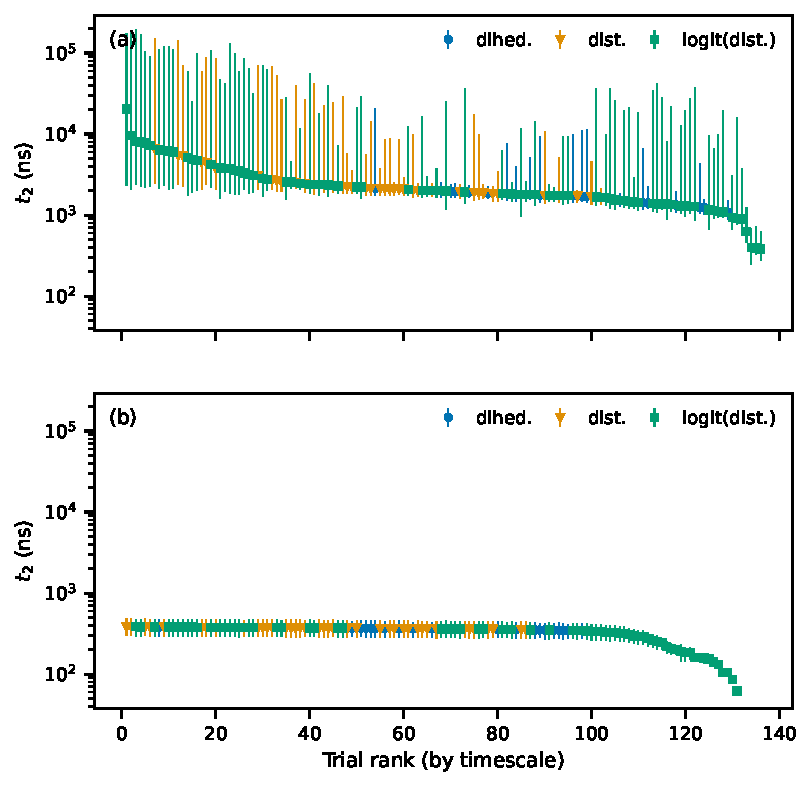
\includegraphics[width=0.7\columnwidth]{results1/timescale_distributions.pdf}
    \caption{\textsc{Timescales of randomly sampled hyperparameter trials.} Panel (a) refers to BBA, panel (b) refers to Chignolin. The vertical axis is the dominant timescale ($t_2$), the horizontal axis is the trial rank. The solid disc and error bars are the median and \SI{95}{\percent} bootstrapped confidence intervals.  }
    \label{fig:random_trials}
\end{figure}


\begin{figure}
    \centering
    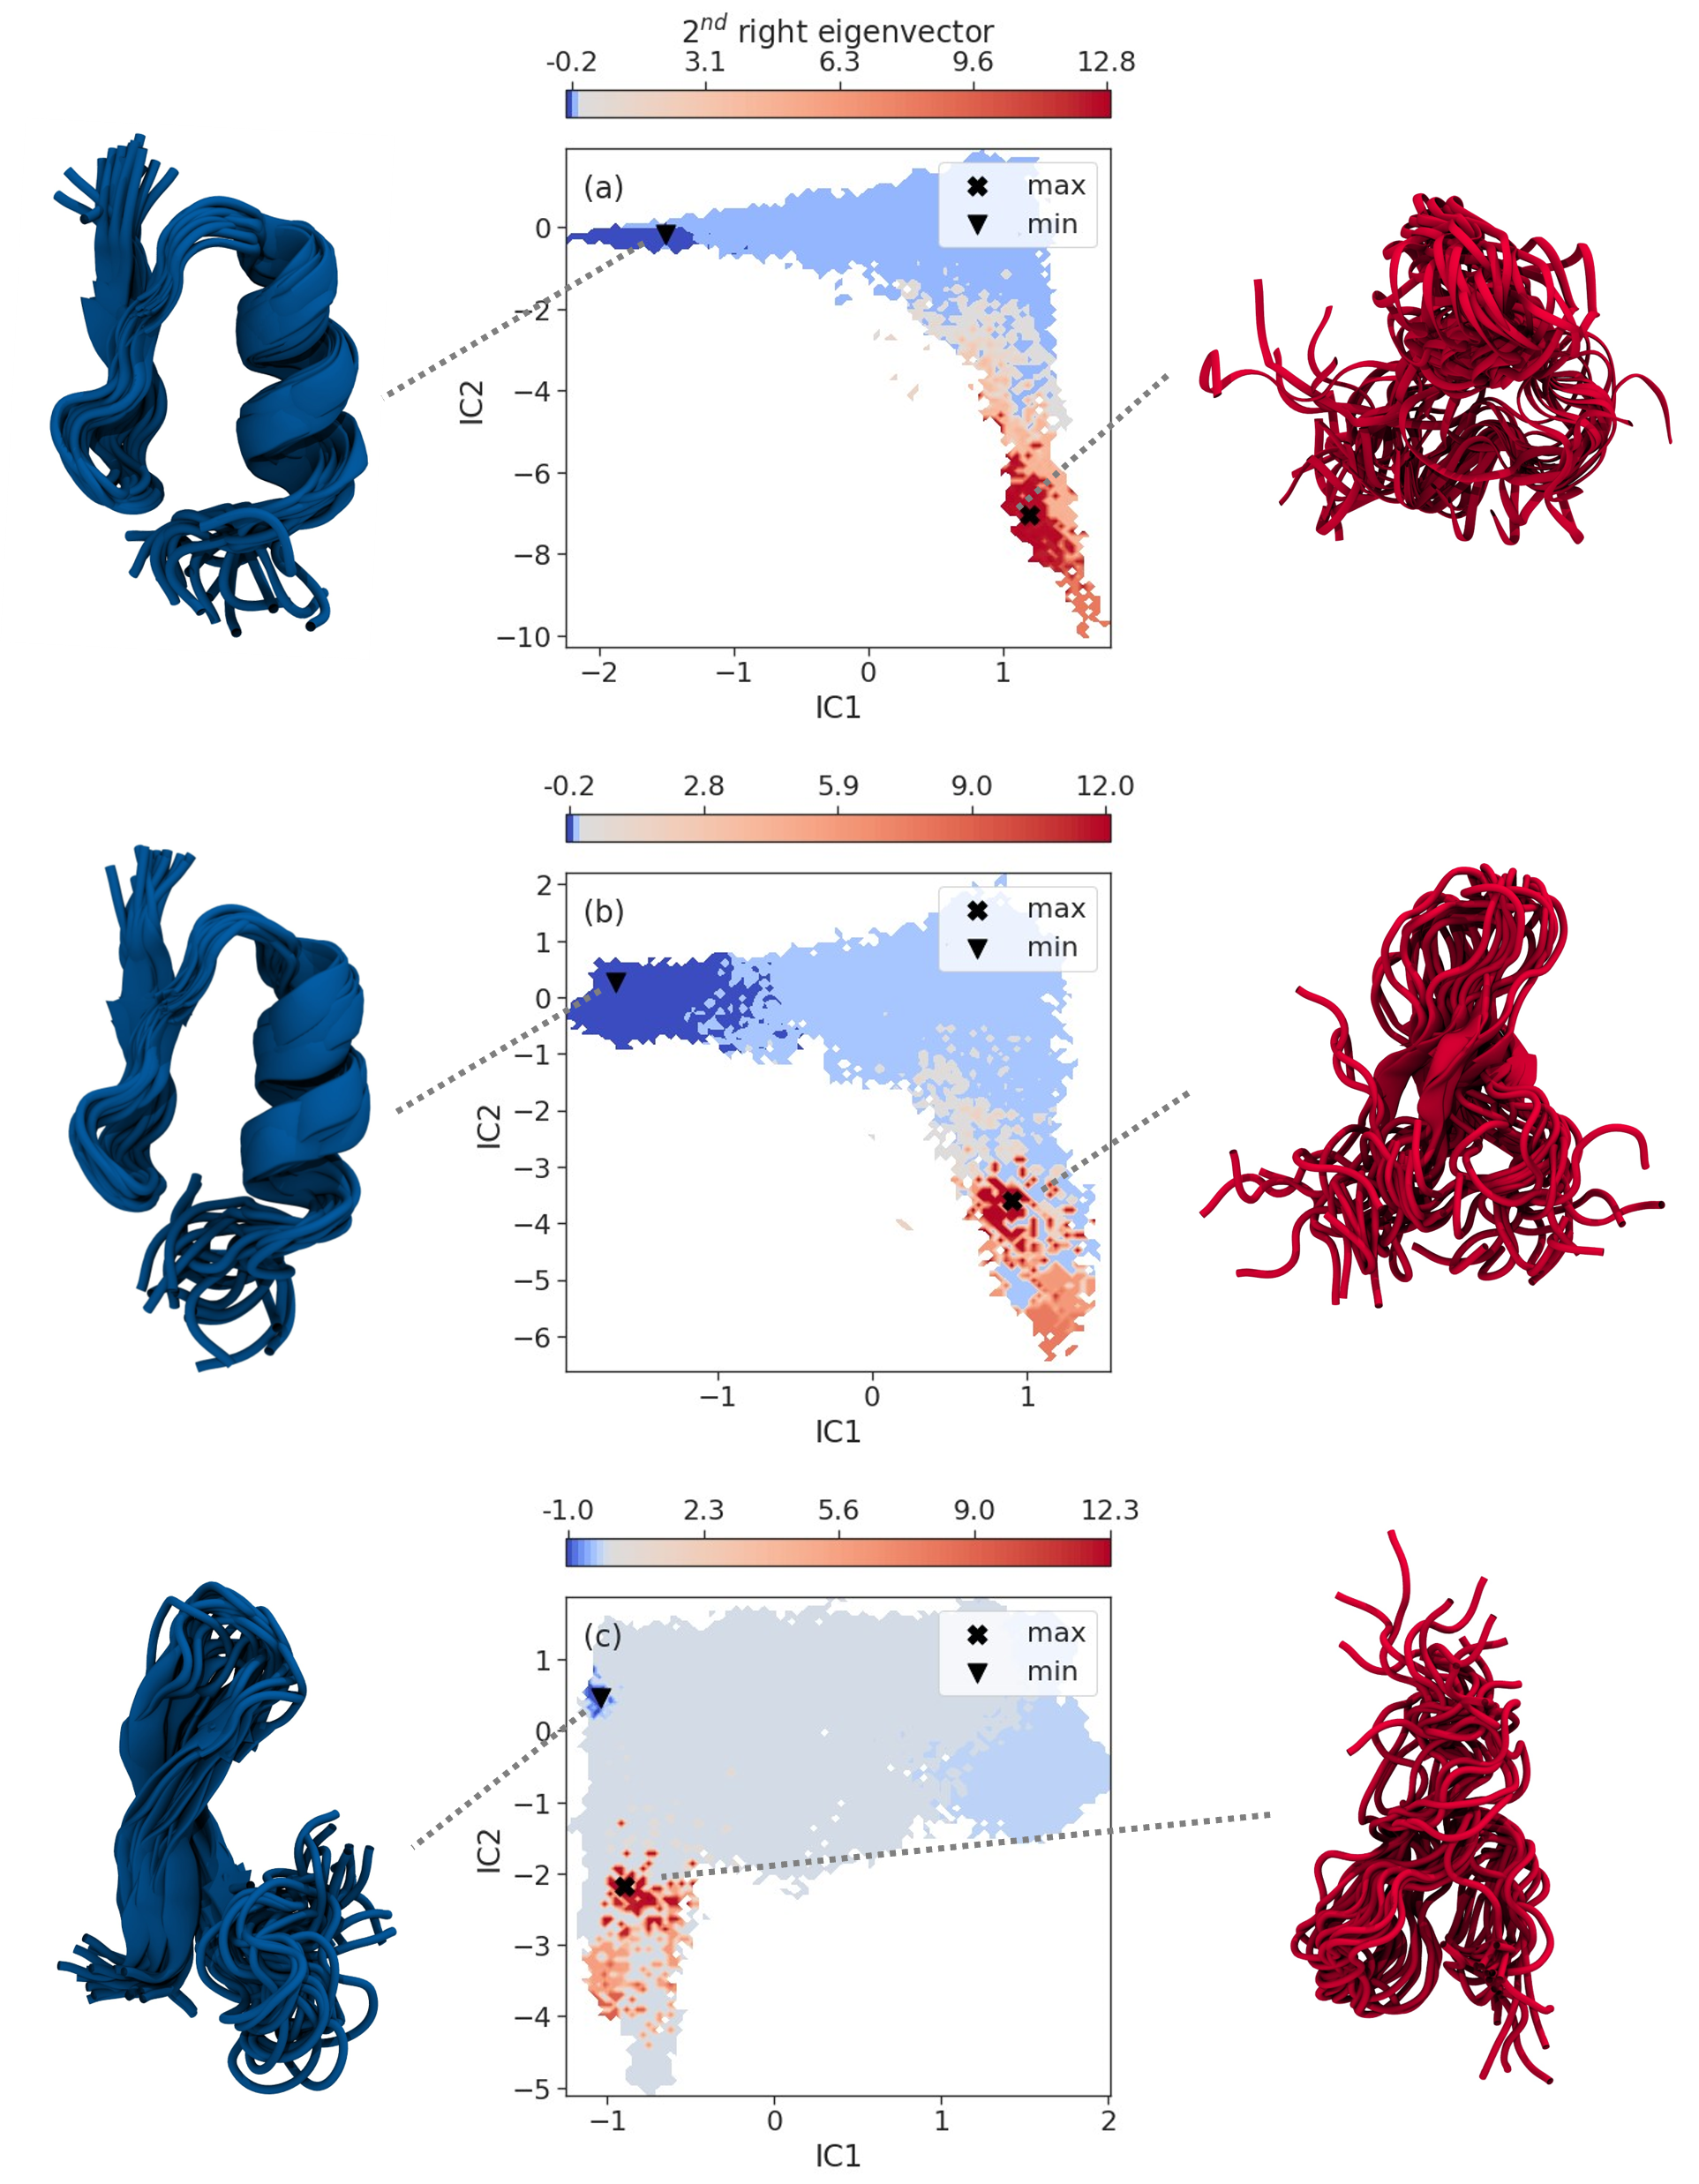
\includegraphics[width=0.7\columnwidth]{results1/different_relaxation.png}
    \caption{\textsc{BBA MSMs with different relaxation processes.} Panel (a) shows the optimi}
    \label{fig:bba_differences}
\end{figure}

Figure \ref{fig:random_trials} shows the distribution of the timescale of the dominant process ($t_2$) for each MSM of BBA (panel (a)) and Chignolin (panel (b)) ordered left to right with highest value of $t_2$ on the left. Each point is colored according to the feature used. According to previous research~\cite{scherer_variational_2019} we expect in both cases that the dominant relaxation process refer to the folded / unfolded transition.  According to the variational theorem the most accurate models (and therefore the `best' set of hyperparameters) are the ones with the largest implied timescales. We would therefore expect that the `best' model would be the model with the highest value of $t_2$. However, implicit in this decision is that the implied timescale represents the same underlying relaxation process. In the case of Chignolin this is the case, as is shown by inspection of the models ranked 1 and 4 (labelled models 1 and 2, see table S1 and sections S2.1 and S2.2).  Despite using different features (distances and logistic distances, respectively) the dominant relaxation processes in both models are similar: figure S3 (c) and figure S6 (c) show conformational ensembles of the extremes of the dominant relaxation process which clearly show similar transitions.  [THIS NEEDS CHECKING].  Given the similarity of $t_2$ for each trial, we expect this observation to generalize to the other hyperparameter trials. 

In the case of BBA, the situation is different. We compared the top two best performing models (ranked 1 and 2 in figure \ref{fig:random_trials}, labeled model 1 and 2 in table S1 and sections S2.4 and S2.5) and the best performing models with the other features: model rank X with the dihedrals feature (model 3, section S2.6) and model rank Y with the distances feature (model 4, section S2.7). 

When comparing model 1 and 2 we see a similar folded-to-unfolded or partially-folded transition represented by the dominant eigenvector (figure \ref{fig:bba_differences} panel (a) and (b)), albeit with different values of $t_2$ (\SIci{20.4}{2.3}{176.2}{\micro\second} cf. \SIci{9.7}{2.1}{188.7}{\micro\second}). The accords with differences in the hyperparameters: model 1 and 2 use the logistic distances features, but model 1 has a logistic transform which is more sensitive to changes in contact distances between \SIrange[range-phrase=---]{0.1}{10}{\angstrom} (see figure S1) and more discrete basis functions (471 cf. 289, see table S1).  

However, inspection of models 3 and 4 show markedly different transitions (figures S18(c) and S21(c) respectively) represented by the dominant eigenvector: both represent different folded-misfolded transitions.  This is to be expected as the features used are different and so we would expect them to pick out different conformational transitions. 

Thus, when optimising MSMs the objective function ($t_2$ in this case) may change definition across the search space and one is not comparing like-with-like when looking at \emph{just} the objective function.  As the largest change in $t_2$ is due to the different features, pre-selecting the feature to use, by for example using the method of Scherer et. al.~\cite{scherer_variational_2019} will be useful. But we also note that one must still select a VAMP lag-time, the differences in the VAMP scores may be small and there may be problems when scoring models using the VAMP2 with equilibrium constraints. 

We therefore suggest that model selection of MSMs by ranking of a single observable be supplemented with inspection of the character of the eigenvectors and other observables, to ensure that one is optimising the intended process. 


\subsection{VAMP2$(k)$ scores of reversible MSMs give inconsistent results}\label{sec:vamps_inconsistent}


\begin{figure}
    \centering
    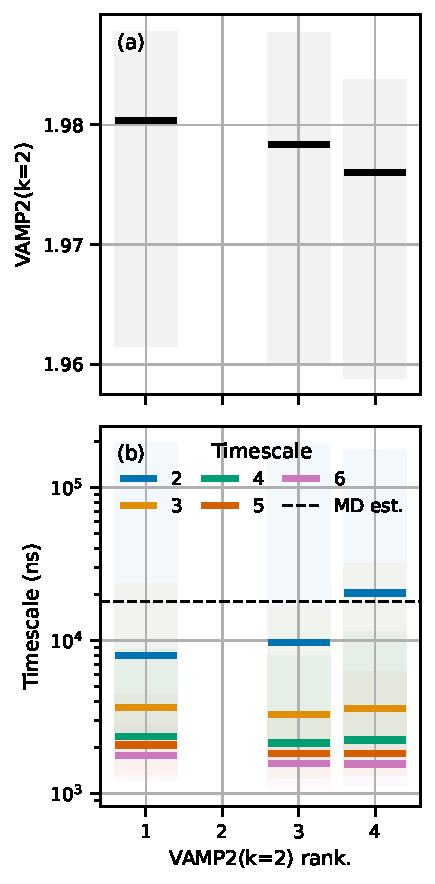
\includegraphics{results2/bad_vamp_ranks.pdf}
    \caption{\textbf{Models with VAMP2$(k)$ scores inversely proportional to timescales}. Panel (a) show the VAMP2$(2)$ scores and panel (b) shows the first five dominant timescales, for a selection of models.  The horizontal axis in both panels is the model rank as judged by the VAMP2$(2)$ score. The selection shows models where the slowest timescale is inversely proportional to the VAMP2$(2)$ score. Models which do not show this correlation are not shown. }
    \label{fig:bad_vamp_scores}
\end{figure}


\begin{figure}
    \centering
    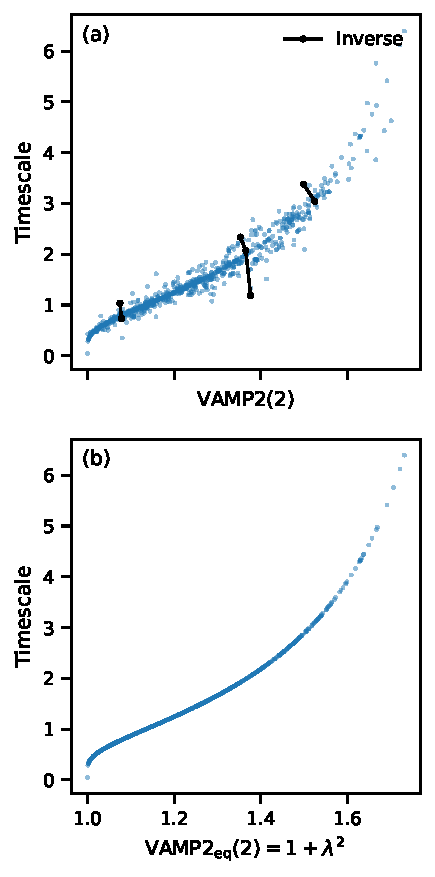
\includegraphics{results2/timescale_vs_vamp_vs_evs.pdf}
    \caption{\textbf{Relationship between implied timescales, t$_2$, VAMP2$(2)$, VAMP2$_{eq}(2)$ scores}.  Each of the \num{1000} blue points is calculated from an MSM estimated from a distinct simulated trajectory of 20 time steps. The trajectories were generated from the same three-state reference transition matrix (taken from Trendelkamp-Schroer et. al.~\cite{trendelkamp-schroerEstimationUncertaintyReversible2015b}). The estimated transition matrices were all estimated ensuring reversibility. Panel (a) shows $t_2$ as a function of VAMP2$(2)$ scores while panel (b) shows  $t_2$ as a function of VAMP2$_{eq}(2)$. The black points labelled `Inverse' are example subsets of MSMs where the relationship between the implied timescale and VAMP2$(2)$ score are inverted.}
    \label{fig:bad_vamps_examples}
\end{figure}


The VAMP2$(k)$ score~\cite{wuVariationalApproachLearning2020c} provide a principled metric for optimising MSM hyperparameters. The benefits are that it can be used for stationary, non-stationary, reversible and non-reversible MSMs. It is linked directly to the kinetic variance captured by the basis states such that maximizing the VAMP2$(k)$ score will maximize the timescales of pertaining to the first $k$ eigenvectors of the model. In addition it can be used with bootstrapping and cross-validation model selection techniques. 

Inspection of the results revealed that for subsets of the trials, VAMP2$(2)$ was inversely proportional to the $t_2$. This is shown in figure~\ref{fig:bad_vamp_scores}. In panel (a) the VAMP2$(2)$ score is shown for the trials ranked first, third, and fourth. In panel (c) the first five timescales are shown for each model.  The dashed line shows the folding timescale from reference~\cite{lindorff-larsen_how_2011}. Timescales for the third to sixth eigenvectors are the same, however $t_2$ clearly \emph{increases} with \emph{decreasing} VAMP2$(2)$ score. The second ranked model is omitted for clarity because it does not follow this pattern. 

We suggest the reason for this behavior is due to the fact by enforcing reversibility in the estimation of the transition matrix it is impossible to get consistency between the three count matrices ($\mathbf{C}_{00/0t/tt}$) and the eigenvectors ($\mathbf{U}/\mathbf{V}$) in equation~\ref{eqn:vamp_def}). 

A similar effect can be seen with a three-state toy model (example 1 from~\cite{trendelkamp-schroer_estimation_2015}). \num{10000} 20-step trajectories were sampled from the same $3\times 3$ transition matrix and for each trajectory count matrices ($\mathbf{C}_{00/0t/tt}$) were estimated.  We assert that the differences in the count matrices arising from the finite sampling in this toy model are similar to the differences from different  discretization schemes in the example of BBA.  From each set of count matrices $t_2$ and VAMP2$(2)$ scores were estimated and  these are shown in figure~\ref{fig:bad_vamps_examples} panel (a). While  $t_2$ is clearly rank-correlated with VAMP2$(2)$, the rank correlation is not perfect.  Many subsets of these results  form sets which are anti-correlated,  three examples of this inverse relationship are shown as black lines labelled `Inverse'. These subsets mirror the effect seen in the BBA models in figure~\ref{fig:bad_vamp_scores}.  As a comparison, panel (b) we plot the sum of the squares of the first two eigenvalues, VAMP2$_{eq}(2)$, which shows perfect rank correlation (as they must). 

The reason for writing the VAMP2$(k)$ score as the product of count matrices and eigenvectors/singular vector matrices is to facilitate data-splitting in cross-validation. While we used bootstrapping for this work and thus mitigate this, the effect of data splitting would be to worsen the discrepancy between the count and transition matrices. This is because the count matrices are now estimated on different data compared to the eigenvector matrices.  

Due to the problems problem of consistency between the matrices in equation~\ref{eqn:vamp_score_def} arising from a) enforcing reversibility and b) data splitting for cross-validation,  \emph{we recommend that VAMP2$(k)$ scores, either cross-validated or bootstrapped, should not used for reversible and stationary MSMs}. Instead we recommend bootstrapping the sum of the squared eigenvalues (VAMP$_{eq}(k)$) directly from the reversible transition matrix. This has the same theoretical properties of the VAMP2$(k)$ score (i.e., represents captured kinetic variance, and link to variational theorem) while not a) wasting data due to data splitting and b) perfect correlation with the implied timescales.


\subsection{Bayesian optimisation can improve timescales}\label{sec:bayes}

\begin{figure}[h]
    \centering
    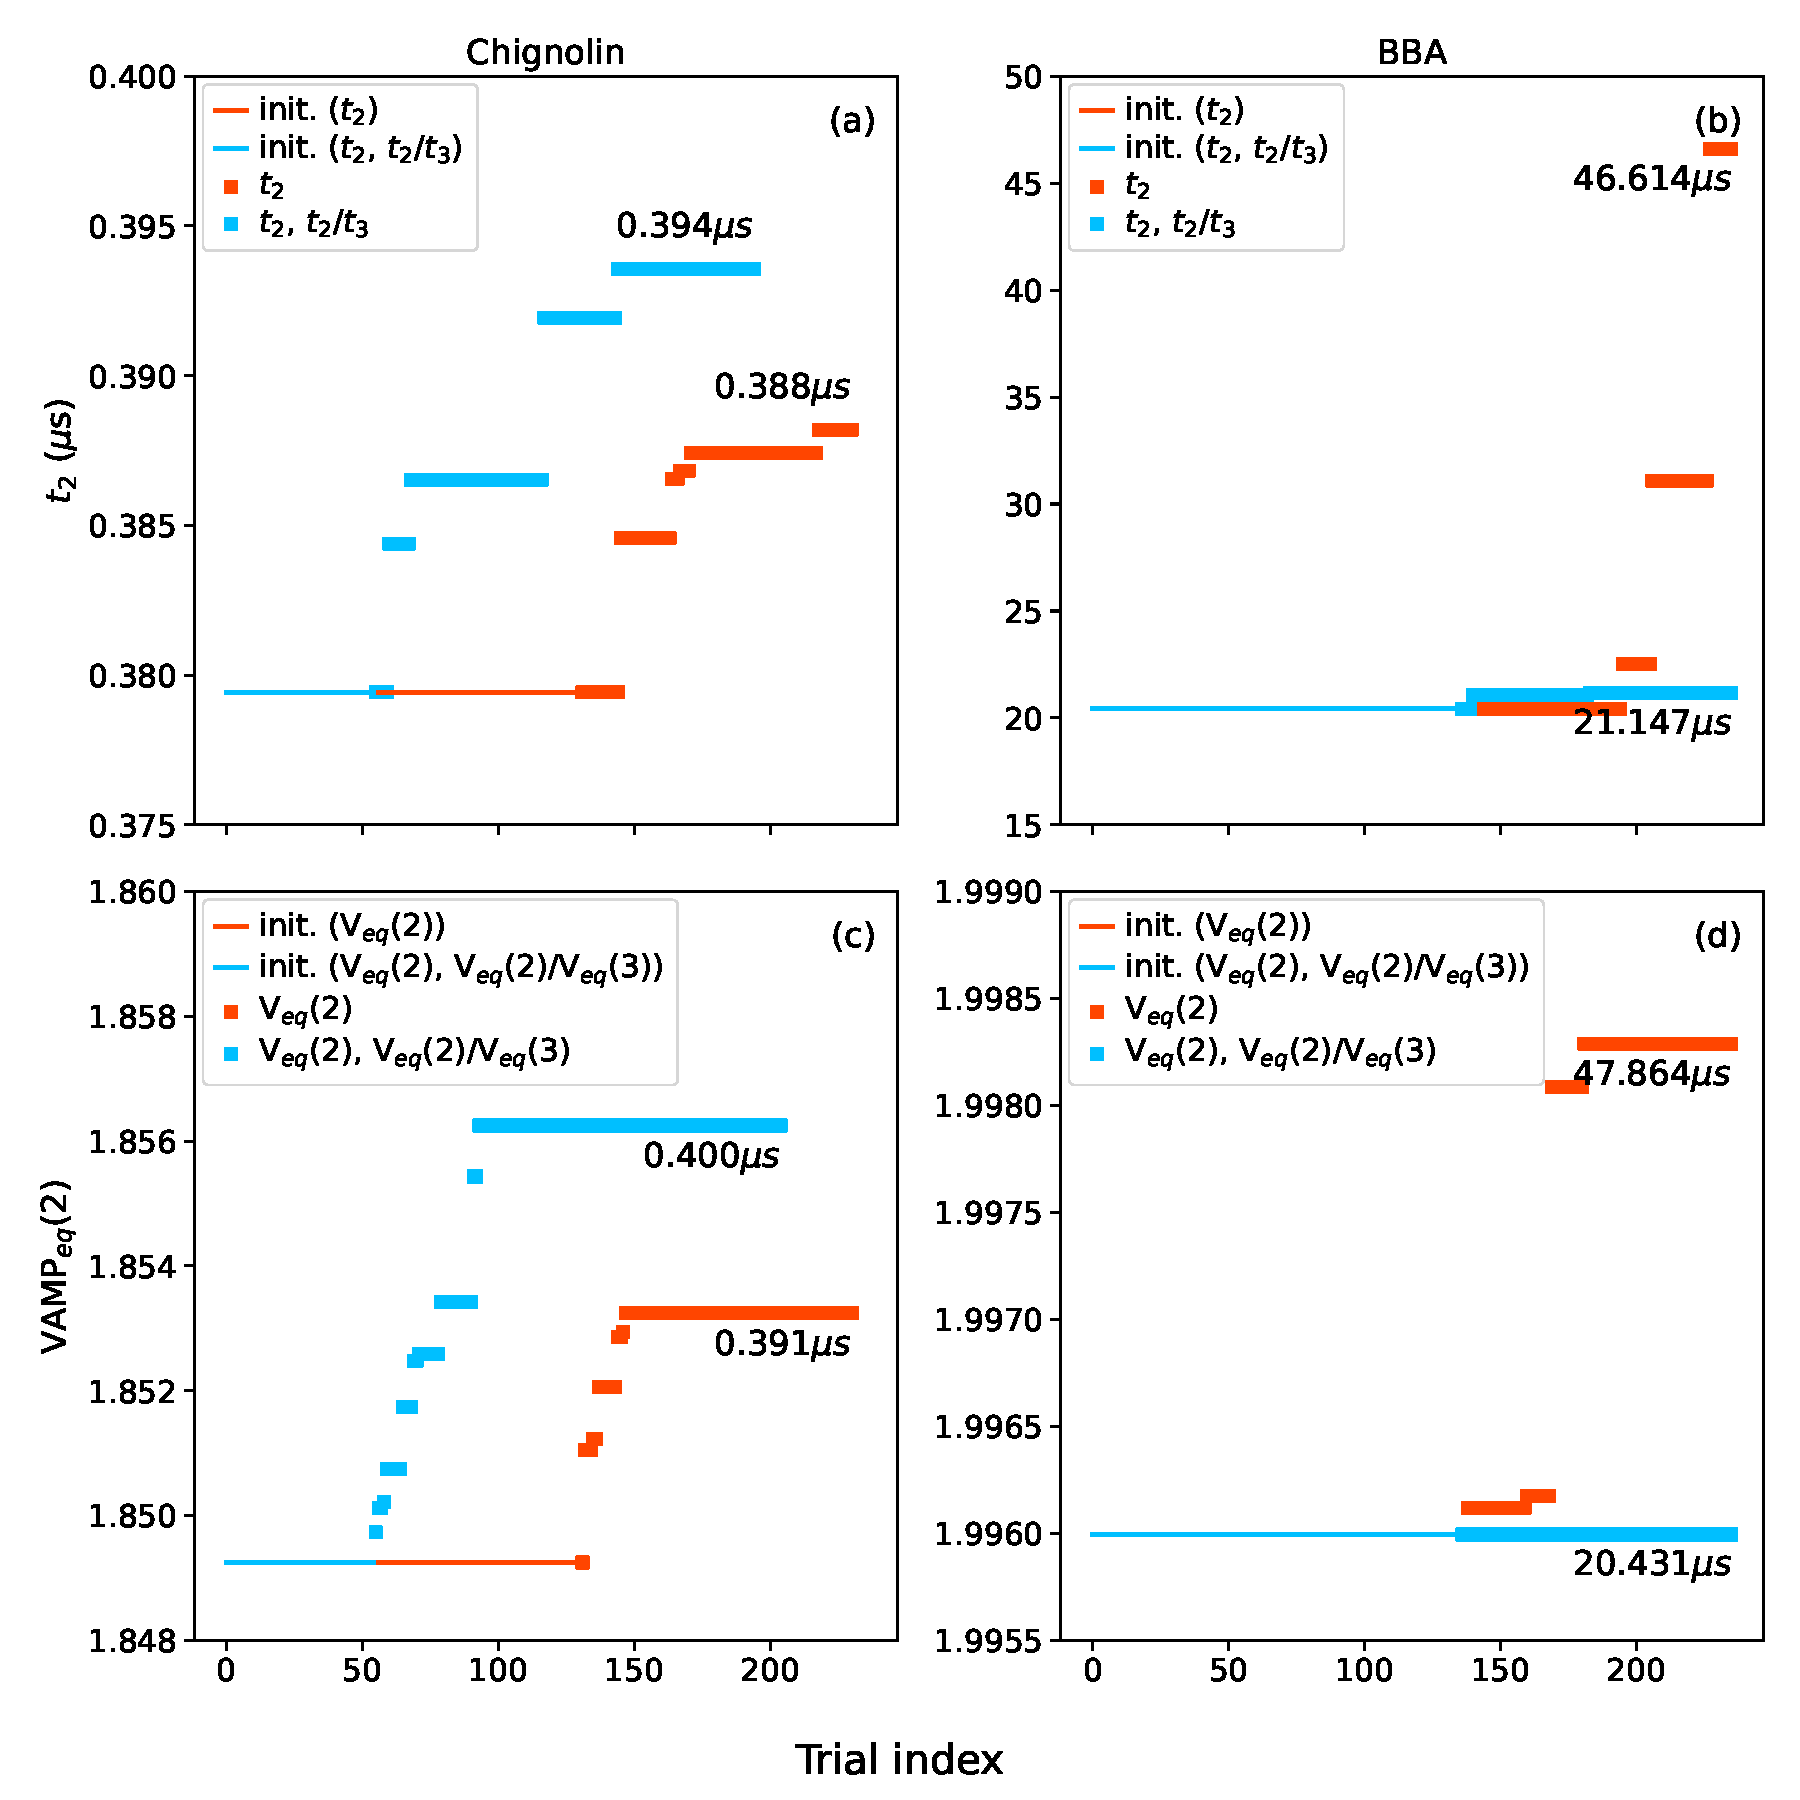
\includegraphics[width=\columnwidth]{results3/optimisation_summary.pdf}
    \caption{\textsc{Optimisation of MSMs of Chignolin and BBA}. The vertical axis is optimisation objective, the horizontal axis is the trial number. The thin line refers to the incumbent over the initialization data (`init.'), the squares are the incumbent at each trial number. Panels (a) and (c) refer to Chignolin, (b) and (d) to BBA. Panels (a) and (b) refer to Bayesian optimisation with either $t_{2}$  (red), or multivariate optimisation of both $t_{2}$ and the timescale gap, $t_{2}/t_{3}$.  Panels (c) and (d) refer to optimisation of  $\mathrm{VAMP}_{eq}(2)$ (red) and multivariate optimisation of both  $\mathrm{VAMP}_{eq}(2)$ and $\mathrm{VAMP}_{eq}(2)/\mathrm{VAMP}_{eq}(3)$. The optimised values of $t_2$ are shown as labels. }
    \label{fig:optimisation_trials}
\end{figure}

We tested whether Bayesian optimisation could increase $t_2$ by selecting better hyperparameters.  We optimised the search space in~\ref{tab:search_space} using both single objective and multi-objective optimisation, with objectives based on the timescales, $t_{2/3}$ and the VAMP$_{eq}(2/3)$ scores, see~\ref{tab:opt_description} for a complete description.  The optimisation using dual objectives of $t_2$ with $t_2/t_3$ (and the VAMP$_{eq}$ equivalent) was prompted by the observation from the randomly sampled hyperparameter trial dataset there were many models with similar values of $t_2$ but with wide range of $t_2/t_3$. A large timescale gap gives rise to models which are more accurate when truncated and coarse grained into a two state model. The results are shown in figure~\ref{fig:optimisation_trials}.  

Single objective optimisation of both $t_2$ and VAMP$_{eq}(2)$ increased $t_2$ for Chignolin and BBA.  For Chignolin the increase was modest, between \SIrange[range-phrase=---]{2.4}{5.5}{\percent} for all four objective functions.  The single objective optimisation of $t_2$ had the smallest increase (panel (a) red squares) while the multi-objective optimisation of the VAMP$_{eq}(2)$ and VAMP$_{eq}(2)$/VAMP$_{eq}(3)$ gave the largest increase in $t_2$ (panel (c) blue squares). 
 
The overall model increase is unsurprising given the consistency of $t_2$ across the randomly sampled hyperparameter trials.  The $t_2$ optimised MSM, model 3 (see table S1 and section S2.3) shows a partially folded to folded transition in figure S9(c) rather than the fully disordered to folded transition in the incumbent.  In terms of the values of the hyperparameters the optimisation has changed the TICA lag-time significantly (the other hyperparameters have remained largely unchanged). 

The VAMP$_{eq}(2)$ and VAMP$_{eq}(2)$/VAMP$_{eq}(3)$ optimised MSM, model 4 (see table S1 and section S2.4) [Something about the MO optimised result.]

Both the dual-objective optimisations ($t_2$ with $t_2/t_3$ and the VAMP equivalent) increased both the $t_2$ and the separation of timescales (see figure S26). 

For BBA the single objective optimisation of $t_2$ and VAMP$_{eq}(2)$ increased $t_2$ by \SI{128}{\percent} and \SI{135}{\percent} respectively.  However, these models have not `optimised' the same relaxation process as the incumbent, model 1. The $t_2$ optimised MSM, model 5 (see table S1 and section S2.8), denotes a transition between two mis-folded structures (see figure S24(c)).  This is perhaps surprising given that the main difference between the two model specification is that change in the logistic transform (see figure S1 for the difference between model 1 and model 5's logistic transform).  

[Something about the V2 + gap optimised model]

Both the dual-objective optimisations ($t_2$ with $t_2/t_3$ and the VAMP equivalent) increased both the $t_2$ and the separation of timescales (see figure S26). 


\subsection{The lag time and number of scored eigenvectors do not affect model selection.}\label{sec:lag_evs_selection}

\begin{figure}[h]
    \centering
    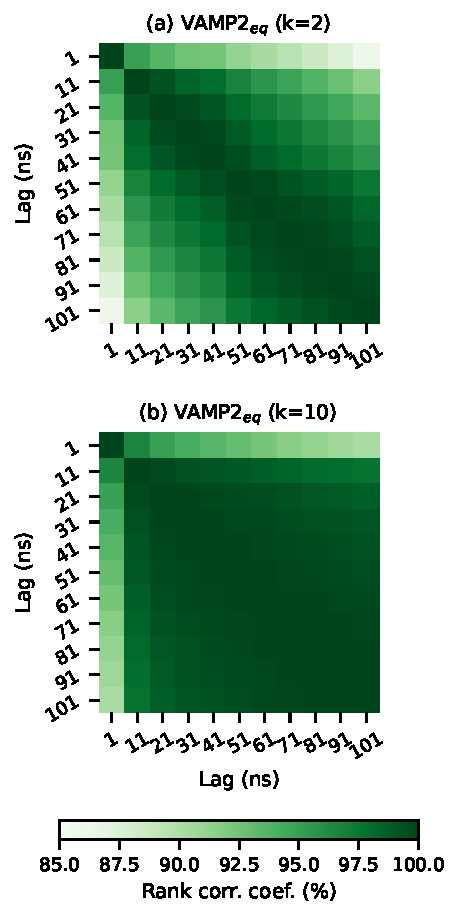
\includegraphics{results4/vampeq_rank_vs_lag.pdf}
    \caption{Consistency of $\operatorname{VAMP2}_{\mathrm{eq}}(k)$ rank with Markov lag time, $\tau$. The $i, j$'th cell in panel (a) shows the Spearman's rank correlation coefficient of $\operatorname{VAMP2}_{\mathrm{eq}}(2)$ for each trial measured at the $i$'th lag time, with  $\operatorname{VAMP2}_{eq}(2)$  measured at the $j$'th lag time.   Panel (b) show the same measurements with $\operatorname{VAMP2}_{\mathrm{eq}}(10)$ score respectively. }
    \label{fig:vamp_rank_vs_lag}
\end{figure}

When evaluating MSMs using a variational score one must specify the both the Markov lag time ($\tau$) and the number of eigenvectors to score ($k$).  However, both these choices affect the VAMP score although it is not clear  whether these choices affect the model ranking. To test how these choices affect model selection we measured the consistency in model rank, as measured by the VAMP2$_{eq}$(k) using the Spearman's rank correlation coefficient, at a) different lag times for given values of $k$ and b) at different numbers of scored eigenvectors at a given lag time. 

Figure~\ref{fig:vamp_rank_vs_lag} shows the consistency between model rankings at different lag times ($\SI{1}{\nano\second} < \tau < \SI{101}{\nano\second}$) with $k=2$ (panel (a)) and with $k=10$ (panel (b)). In addition, scatter plots of the data used to calculate these coefficients for $k=2, 3, 5, \&\ 10$ are shown in the supplementary information figures~\ref{fig:vampeq2_rank_vs_lag_pairplot} to \ref{fig:vampeq10_rank_vs_lag_pairplot}.  Across all lags and for both small ($k=2$) and large ($k=10$) numbers of scored eigenvectors, the consistency in the model ranking is high (greater than \SI{85}{\percent}). The consistency between models with lag times greater than $\tau=\SI{1}{\nano\second}$) is much greater, with rank correlations up to \SI{100}{\percent}.  This effect is most pronounced for $k=10$ scored eigenvectors. In particular, good consistency is achieved at lag times smaller than those required for the model to be Markovian ($\tau=\SI{41}{\nano\second}$).


\begin{figure}[h]
    \centering
    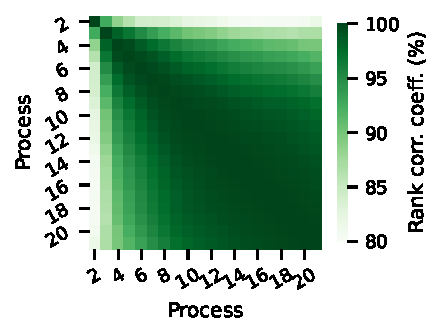
\includegraphics{results4/vampeq_rank_vs_proc.pdf}
    \caption{\textsc{Consistency of $\operatorname{VAMP2}_{eq}(k)$ rank with number of scored eigenvectors}. The ranks of trials in the row $k$ are compared to their rank at the column $k$ using the Spearman's rank correlation coefficient at a lag time of \SI{41}{\nano\second}}
    \label{fig:vampeq_rank_vs_n_procs}
\end{figure}

Figure~\ref{fig:vampeq_rank_vs_n_procs} shows the consistency between model rankings at different number of scored eigenvectors ($2 < k < 21$) at a lag time of \SI{41}{\nano\second} (the value used in all previous analysis). Again, the consistency is generally high with a rank correlation between all pairs of $k$ of at least \SI{80}{\percent}. The ranking is most consistent between values of $k$ larger than \num{4}.  From these two analyses taken together, we see that for long lag-times and large number of scored eigenvectors model ranking is not affected by the choice of $\tau$ and $k$.

\section{Conclusions}

This work has shown that automated MSM optimisation should be approached with caution.  Changing they hyperparameters, even slightly, can give rise to different processes, making comparison between functions of the eigenvalues (e.g., timescales, VAMP/GMRQ scores) meaningless.  

Using VAMP scores for reversible MSMs should be also be approached with caution.  Other options, such as bootstrapped observables ($t_2$) relate more directly to model observables and can also be used to rank models.  

Given these to observations, it is imperative the a range of different hyperparameters should be trialled and the results reported, in line with good statistical practice.  

Bayesian optimisation  works? Doesn't work? 

however, the lag time and the number of scored eigenvectors does not appear to change the ranking of the models (according to the VAMPeq).  

Taken together these observations suggest a nubmer of recommendations: 

\begin{enumerate}
    \item Random sample a range of hyeparmaeetes and inspect the results for the consistency of the eigenvectors.  
    \item Use the VAMPeq or $t_2$ to rank hyperparameters. 
    \item The lag time and the number of scored eigenvectors in VAMPeq do not affect model ranking, so it is not as important to test these in the range of models tested. 
\end{enumerate}



% This work has answered a number of questions pertaining to selecting hyperparameters for discrete MSMs.  We have seen that the type of feature plays an important role but that the other hyperparameters need to be chosen carefully to optimize the implied timescales.  The sensitivity of the implied timescales is generally low, meaning small variations in their values do not change the timescales significantly.  However, the relative sensitivity of the non-feature hyperparameters changes depending on type of feature used: e.g., with some features the number of microstates is most important while with others the timescales are not affected.  The VAMP variational scores, which have recently been used to perform model selection on reversible MSMs have been shown to give results which are not in line with the assumed variational principle underlying them. 

% Given this relatively complex picture of hyperparameter optimisation we recommend the following for optimising reversible MSMs: 

% \begin{enumerate}
%     \item \textbf{A number of different features should be tried}. They can be selected from a list, potentially informed by the VAMP scores developed for by Schrere et. al. \cite{scherer_variational_2019}. 
%     \item \textbf{Remaining hyperparameters should be randomly sampled from a suitable search space}. Using a grid search method is inefficient and not easily modified to sample more hyperparameters,  if necessary. 
%     \item \textbf{Score models using bootstrapped VAMP2$_{eq}(k)$}. This is preferable to using the VAMP2$(k)$ variational score because they can lead to contradictory results. 
%     \item \textbf{If the MSM requires significant resources to estimate, Bayesian optimisation may be a useful tool}.  This work used a Gaussian process surrogate model but other, more flexible models may perform better (see limitations discussion below). 
%     \item \textbf{Bayesian optimisation provides a principled way of checking the convergence the model}.  Even if the the MSM does not require significant resources, we suggest reporting an optimized model and a set of models which make it clear that the behaviour of model observables is consistent with variation in the hyperparameters. 
%     \item \textbf{When scoring the models use as many eigenvectors as are resolvable}. This can be estimated from a selection of models or all processes can be scored and saved in a database (as was performed here).  
%     \item \textbf{For model selection, it is not important to select a `Markovain' lag time}. However, for efficiency reasons, this should be attempted to be estimated from a selection of models.  
% \end{enumerate}

% There are a two main limitations of this study.  First the we have a performed our analysis on only one system which limits the applicability some of the specific results. For example, the sensitivity of the hyperparameters to the timescales should be not taken as generally applicable for other systems. Second, the fitting of the Gaussian process used in the sensitivity calculation and the Bayesian optimisation required a lot of ad-hoc preprocessing and its own model selection procedure.  More flexible models which still return estimates of input importance and of uncertainty, such as random forests or tree parzen estimators, may be more appropriate see for example [] and [].   



%%%%%%%%%%%%%%%%%%%%%%%%%%%%%%%%%%%%%%%%%%%%%%%%%%%%%%%%%%%%%%%%%%%%%
%% The "Acknowledgement" section can be given in all manuscript
%% classes. This should be given within the "acknowledgement"
%% environment, which will make the correct section or running title.
%%%%%%%%%%%%%%%%%%%%%%%%%%%%%%%%%%%%%%%%%%%%%%%%%%%%%%%%%%%%%%%%%%%%%
\begin{acknowledgement}

Please use ``The authors thank \ldots'' rather than ``The
authors would like to thank \ldots''.


\end{acknowledgement}

%%%%%%%%%%%%%%%%%%%%%%%%%%%%%%%%%%%%%%%%%%%%%%%%%%%%%%%%%%%%%%%%%%%%%
%% The same is true for Supporting Information, which should use the
%% suppinfo environment.
%%%%%%%%%%%%%%%%%%%%%%%%%%%%%%%%%%%%%%%%%%%%%%%%%%%%%%%%%%%%%%%%%%%%%
\begin{suppinfo}


\end{suppinfo}

%%%%%%%%%%%%%%%%%%%%%%%%%%%%%%%%%%%%%%%%%%%%%%%%%%%%%%%%%%%%%%%%%%%%%
%% The appropriate \bibliography command should be placed here.
%% Notice that the class file automatically sets \bibliographystyle
%% and also names the section correctly.
%%%%%%%%%%%%%%%%%%%%%%%%%%%%%%%%%%%%%%%%%%%%%%%%%%%%%%%%%%%%%%%%%%%%%
\bibliography{references.bib}
%\bibliography{bibliography.bib}

\end{document}





% \begin{itemize}
    % \item Markov state models are a popular model for analysing MD data. 
    % \item They are able to provide a quantitative picture of the conformational dynamics of biomolecular systems. 
    % \item They have been used to study protein folding, ligand binding, peptide- and protein-protein association,  enzymatic reaction dynamics. 
    % \item They have also been used in adaptive sampling algorithms where statistical properties of the model are used to select conformations from which to seed more MD simulations to speed convergence. 
    % \item Like any any statistical model, a number of choices must be made when estimating an MSM. These include choice of estimation algorithm, convergence criteria for optimizing loss-functions; batching, sub-sampling and splitting data for compute resource management and estimating out of sample accuracy; data pre-processing e.g., image resizing, feature-scaling and warping; feature selection and egineering, de-correlating etc. 
    % % \item These choices affect the outcome of the model to varying to degrees but are not `learned' from the data via minimizing a loss function, in the way the parameters of the model are (e.g., neural network weights, MSM transition matrix elements). For this reason they are called `hyperparameters' of the model. 
    % \item There has been a lot of recent attention paid to the affects of hyperparameter selection in, for e.g.,  psychology, neuroscience and machine learning  where opaque methods of hyperparameter selection have lead to irrepreducible results. 
    % \item There are a host of different approaches to this problem, which differ according to whether explanatory power or predictive accuracy of the model are required. 
    % \item When statistical models are made for their explanatory power variants of sensitivity analysis are often used. SA entails estimating models with  several plausible sets of hyperparameters to see how they affect the results [ref].  Similarly, multiverse analysis uses a more thorough enumeration of potential hyperparameters [ref].  Specification curve analysis [ref] also uses a multiverse of results while going further to infer information from the distribution of results. 
    % \item In machine learning, where predictive power is often more important, hyperparameters can be chosen to optimize performance metrics of the model, e.g., out of sample accuracy. Hyperparameters can be randomly or uniformly selected, or even optimized using e.g., Bayesian optimisation.  
    % \item The essential task in MSM estimation is to choose hyperparameters for preprocessing MD data into a smaller number of basis  states for which the MSM can be estimated. 
    % \item traditionally these basis states are discrete states corresponding to small regions of configuration space of the protein. Recent work has focused on estimating fuzzy basis sates using deep learning approaches.  
    % \item Either way a number of hyperparameters must be chosen. The resulting basis states can be judged according to variational scores. 
    % \item For reversible MSMs the generalized matrix Rayleigh coefficient (GMRQ) was introduced as metric of optimising basis states.  This was later expanded to include non-reversible and non-stationary MSMs with the variational approach to Markov processes (VAMP). 
    % \item By varying hyperparameters to increase the variational score, the basis states can be made increasingly accurate. 
    % \item  However, most recent papers which utilise MSMs as their man analytic tool, do not report how hyperparameters were chosen.  
    % \item Where methods for hyperparameter selection were discussed VAMP scores were generally used to discriminate between a handful of different hyperparameters.  
    % \item Taking inspiration from the literature on sensitivity analysis and hyperparameter optimisation we investigate whether more extensive hyperparameter selection methods are needed or appropriate. 
    % \item We investigate how sensitive how MSM timescales are to changes in hyperparameters, demonstrate how an active learning approach might work to finding good quality hyperparameters might work and comment on the commonly used VAMP scores for optimizing basis states.
    % \item This work is structured as follows. Section~\ref{theory} covers the theory of Markov state models and of hyperparameter optimisation and search strategies; section~\ref{methods} covers the methods and materials used; section~\ref{results} discusses results using the fast folding protein BBA as an example; section~\ref{conclusion} concludes with recommendations for estimating MSMs. 
% To get a sense of the current practice for estimating MSMs a small survey of recent literature was conducted. Web Of Science[] was used to look for articles citing PyEMMA~\cite{schererPyEMMASoftwarePackage2015a}, Enspara~\cite{porter_enspara_2019} and MSMBuilder~\cite{beauchamp_msmbuilder2:_2011} and Deeptime~\cite{deeptime}, published since 2020 and 25 randomly selected for detailed investigation~\cite{tosstorff_study_2020, fernandez-quintero_mutation_2021, kahler_sodium-induced_2020, paul_thermodynamics_2021, quoika_implementation_2021, liu_misfolding_2020, tian_deciphering_2020, hempel_molecular_2021, koulgi_structural_2021., sharma_comparative_2020, mckiernan_dynamical_2020, dutta_distinct_2022, zhou_molecular_2021, fernandez-quintero_cdr_2022, song_modulation_2021, sadiq_multiscale_2021, ibrahim_dynamics_2022, linker_polarapolar_2022, hu_discovery_2022, cannariato_prediction_2022, jones_determining_2021, zhu_critical_2021, zhu_critical_2021, bergh_markov_2021, pantsar_decisive_2022, grabski_molecular_2021}. Articles looking at purely methodological questions were excluded. Three questions were asked: 
% \begin{itemize}
%     \item Were sensitivity analyses performed? i.e., were the sensitivity of observables tested with respect to the model hyperparameters?
%     \item How did the authors select the hyperparameters? e.g., using VAMP score? 
%     \item Did the authors perform a validation of the selected model using implied timescales and/or a Chapman-Kolmogorov test? 
% \end{itemize}

% Only one of the studies presented a sensitivity analysis, (this analysis also served as a hyperparameters selection technique)~\cite{bergh_markov_2021}. The the majority (15, \SI{60}{\percent}) of studies did not discuss any hyperparameter search techniques and of those that did,  the majority~\cite{paul_thermodynamics_2021, koulgi_structural_2021, sharma_comparative_2020, dutta_distinct_2022, zhou_molecular_2021, jones_determining_2021, zhu_critical_2021, grabski_molecular_2021} used VAMP scores (8, \SI{89}{\percent}), while one article used the elbow method with important observables \cite{bergh_markov_2021} as their objective function. Only a minority~\cite{quoika_implementation_2021, hempel_molecular_2021, song_modulation_2021, ibrahim_dynamics_2022} failed to give evidence of validation.  

% It can be concluded that hyperparameter optimisation is popular but not universal and sensitivity analysis is either a) not performed or b) not thought important (either by journals or by the authors) enough not to include in the journal article. 
% \end{itemize}





% \begin{itemize}
%     \item The variational theorem applied to the transfer operator $\mathcal{T}(\tau)$, implies that the sum eigenvalues of the $\mathbf{T}$ in some arbitrary basis, will always be less than the sum of the true eigenvalues. 
%     \item Thus, one is free to choose a basis which will increase the sum of the eigenvalues. The associated timescales and eigenvectors will become closer to the true timescales and eigenvectors. 
%     \item In practice we restrict the score to pertain to the $k$ slowest processes, where $k=2 - \simeq 10$. We write the score as $S(\bm{\theta}; k) = \sum_{i=1}^{k}\lambda_{i}$. The functional dependence on $\bm{\theta}$ highlights the fact that the score is assessing the accuracy of the basis states. 
%     \item A general method of finding the most accurate basis states would be to vary the elements of $\bm{\theta}$ until a sufficiently large value of $S$ is found.  However, as pointed out in [mcgibbon] this would favour basis states which fit to noisy fluctuations in the data and do not represent the most accurate basis states, i.e., they would over-fit to the data at hand.
%     \item There are two common techniques to avoid over-fitting. First is the Bootstrap [ref bootstrap] and Cross-validation. The approach  taken by [Noe] and [Pande] is to use cross-validation. 
%     \item The cross-validated estimator of $S$ first estimates the eigenvectors on half of the discretized MD data (the matrix of eigenvectors is given by $\mathbf{U}^{i}$, where the $i$ denotes the $i$th training cross-validation split) the count ($\mathbf{C}_{01}^{-i}$, where $-i$ denotes the complementary test split to $i$) and population ($\mathbf{C}_{00}^{-i}$) matrices are estimated on the remaining half of the data. This is repeated $N$ times with the score being given by: 
%     \begin{equation}
%         GMRQ(\bm{\theta}; k) = \frac{1}{N}\sum_{i}^{N} \operatorname{Tr}\left[(\mathbf{U}^{iT}\mathbf{C}_{01}^{-i}\mathbf{U}^{i})(\mathbf{U}^{iT}\mathbf{C}_{00}^{-i}\mathbf{U}^{i})^{-1}\right]
%     \end{equation}\label{eqn:gmrq_cv_def}
%     \item In other words, this tests how well the training eigenvectors, diagonalize the test count and population matrices. 
%     \item Because the eigenvectors are estimated from a reversible transition matrix they are not consistent with the count matrix.  To account for this, a symmetrized count matrix is used: $\mathbf{C}_{01}^{\mathrm{rev}} = \mathrm{T}^{\mathrm{rev}}\cdot \bm{\Pi}^{\mathrm{rev}}$.  Where $\Pi$ is a diagonal matrix with the elements of $\pi$ on its diagonal. 
%     \item The VAMP scores follow the same principle as the GMRQ but with a distinction drawn between populations at time $t$ and at time $t+\tau$. I.e., $\mathbf{C}_{00} \neq \mathbf{C}_{11}$
%     \item this is to allow the possibility of non-stationary and non-reversible models.
%     \item Instead of eigenvectors, left and right singular vectors, $\mathbf{U}$ and $\mathbf{V}$ of the transition matrix are used (the cross-validation notation is dropped for clarity): 

%     \item When the count and population matrices and the singular vectors are all estimated from the same data, this amounts to the sum of the singular vectors raised to the power of $r$.  
%     \item When $\mathbf{C}_{00} = \mathbf{C}_{11}$ and $\mathbf{C}_{01}$ symmetric, then this expression with $r=1$ should be equivalent to the GMRQ.  i.e., the singular values should equal the eigenvalues.  
%     \item With $r=2$ this expression measures the kinetic variance~\cite{noeKineticDistanceKinetic2015} captured by the basis sets. 
%     \item Both scores truncate the eigenvector/singular vectors to the first $k$ components to restrict the score to just those processes. 
%     \item Both formulae can also be used with bootstrapping where the train and test data are the same but $N$ data sets are generated by sampling with replacement from the pool of available MD trajectories.   
%     \item The VAMP-r scores have also been adapted to score the features only [ref]. 
% \end{itemize}


Theory


SENSITIVITY ANALYSIS

Sensitivity analysis is used to determine the dependency of model outputs on their inputs [uncertainty book]. This is a large research area and we refer the reader to [uncertainty book] and the references within for a full account.  In this work, we conduct a \emph{global sensitivity analysis} which looks at model outputs as a function of the whole input space. This is in contrast to a \emph{local sensitivity analysis} which look at  how small perturbations around a give set of inputs affect the outcomes.  Our simplified sensitivity analysis is based on the work of [bergstra] which modelled the accuracy of a deep neural network image classifier in response to changes in its hyperparameters (e.g., the learning rate) as Gaussian process.  

The sensitivity of the hyperparameters are calculated from the learned parameters of the covariance matrix, specifically the values of $l$ for each term in equations~\ref{eqn:plus_kernel} or \ref{eqn:mult_kernel}.  $l_{i}$  determines how correlated the response is as a function of the distance between two different points of the $i$'th hyperparameters $\theta^{i}$. For a large value of $l_{1}$, two observations $y_{i}, y_{j}$ will be, on average, correlated with one another for a given large values of $|\theta_{i}^{1} - \theta_{j}^{1}|$. This means $y$ does not vary significantly with changes in $\theta^{1}$. The converse will also be true: for small $l_{1}$, $y$ will change significantly for given large value of $|\theta_{i}^{1} - \theta_{j}^{1}|$. Thus, the sensitivity of the response to hyperparameter $i$ can be measured by the \emph{relevance}, $R_{i}$: 
\begin{equation}\label{eqn:relevance_def}
    R_{i} = \frac{1}{l_{i}}
\end{equation}

A popular type of model based search is Bayesian optimisation. The Bayesian optimisation algorithm is applied to MSM estimation is as follows: 

\begin{enumerate}
    \item Randomly sample a small set of hyperparameters and measure the response of the resulting MSMs. This gives a hyperparameter trial data-set $\mathcal{D}_{n}=\left\{(y_1, \bm{\theta}_1),  \ldots (y_n, \bm{\theta}_n) \right \}$ where $y$ is the model response.
    \item Fit a regression model called a \emph{response surface}, which predicts $y$ as a function of $\bm{\theta}$ using the data $\mathcal{D}$: $y \simeq \hat{S}(\theta) + \epsilon$ (where $\epsilon$ is some error term). 
    \item \label{step:calc_alpha} Calculate an acquisition function, $\alpha$, which is a function of the response surface: $\alpha=\alpha\left[\hat{\bm{\theta}}\right]$. The acquisition function maps the hyperparameters to their utility towards optimising $y$. In other words, it suggests hyperparameters that are likely to optimize $y$. 
    \item Use $\alpha$ to suggest a set of hyperparameters, $\bm{\theta}_{n+1} = \argmax_{\bm{\theta}}{\left[\alpha(\hat{S})\right]}$ and measure the response, $y_{n+1}$ by fitting the MSM.  
    \item \label{step:reestimate_rs} Re-estimate the response surface with the new observations incorporated into the trial data-set, $\mathcal{D}_{n+1}$
    \item Repeat steps~\ref{step:calc_alpha} to \ref{step:reestimate_rs} until convergence is reached in the variational score. 
\end{enumerate}

Gaussian process regression models  are popular as response surface models and these will be discussed below. There are many different acquisition functions, in this work we use the expected improvement.  The improvement, $I$, is the one-sided difference between the current best trial value, called the incumbent, $y^{*} = \max_{\bm{\theta}\in \mathcal{D}}{S(\bm{\theta})}$ and a value of the score: $I(\bm{\theta}) = \max{\left(\hat{S}(\bm{\theta}   -y^{*}, 0\right)}$. The expected improvement is the expectation of this value after integrating out the uncertainty in the response surface $\hat{S}$. It takes into account both the size of the improvement and its probability of occurring. 

\subsubsection{Gaussian process regression}

Gaussian process regression (GPR) models an outcome, $y$, (in our case the variational score) as a function of inputs, $\bm{\theta}$, (in our case a vector representing the MSM hyperparameters) in the form of a multivariate normal distribution: 
\begin{equation}
   y = \hat{S}(\bm{\theta}) \sim \mathcal{N}\left(\mu(\bm{\theta}), \mathbf{K}\right ) \label{eqn:gp_def}
\end{equation}
where $\mu(\bm{\theta})$ is the mean function and $\mathbf{K}$ matrix which specifies the covariance between different, arbitrary, values of the outcome, $y$ at different values of $\bm{\theta}$. To understand this expression, first specifying a set of points of $\bm{\theta}$ and a value of $\mu$, e.g., $\mu=0$. Then sampling from the resulting multivariate normal distribution gives rise to a mapping between $\bm{\theta}$ and $y$.

However, as written, equation~\ref{eqn:gp_def}, contains no information.  To make predictions about new points, $(y_{*}, \bm{\theta}_{*})$ (the asterisk denotes unseen data), training data $\mathcal{D}_{n}=\left\{(y_1, \bm{\theta}_1),  \ldots (y_n, \bm{\theta}_n) \right \}$,  needs to be incorporated into the definition of  $\mu$ and $\mathbf{K}$:  

$$
\begin{aligned}
\mu & =K\left(\bm{\theta}_*, \bm{\theta}\right)\left[K(\bm{\theta}, \bm{\theta})+\sigma_n^2 I\right]^{-1} \mathbf{y} \label{eqn:gpr_pred_mu} \\
\mathbf{K} &=K\left(\bm{\theta}_*, \bm{\theta}_*\right)-K\left(\bm{\theta}_*, \bm{\theta}\right)\left[K(\bm{\theta}, \bm{\theta})\right]^{-1} K\left(\bm{\theta}, \bm{\theta}_*\right), \label{eqn:gpr_pred_cov}
\end{aligned}
$$
here $K\left(\bm{\theta}_*, \bm{\theta}\right)$ is the covariance between the response at some arbitrary new points, $\bm{\theta}_*$, and the points in training data $\bm{\theta}$ (and similarly $K\left(\bm{\theta}_*, \bm{\theta}_*\right)$, and $K\left(\bm{\theta}, \bm{\theta}\right)$). The GPR model thus specified predicts a response $y_*$, given a new set of inputs, $\bm{\theta}_*$, as a Gaussian distribution, with a mean and variance derived from equations~\ref{eqn:gpr_pred_mu} and~\ref{eqn:gpr_pred_cov}. 

In order to calculate the covariance between the response in the training data and the response of new points, a covariance kernel is used. As an example, equation~\ref{eqn:gauss_kernel} shows the Gaussian kernel: 
\begin{equation}
    k(\theta_i, \theta_j; l) =  \exp\left(-\frac{\left|\theta_i-\theta_j\right|^2}{l^2}\right), \label{eqn:gauss_kernel}
\end{equation}
it calculates the covariance between the response $y_i$ and $y_j$ with input values of $\theta_i$ and $\theta_j$. It is parameterized by a length-scale parameter, $l$, which is learned from the training data. To increase the flexibility of the covariance calculation, equation~\ref{eqn:gauss_kernel} can be augmented to: 
\begin{align}
    K(\theta_i, \theta_j) & = \eta^2  k(\theta_i, \theta_j; l) + \sigma^2\delta_{ij}, 
\end{align}
here $k(\theta_i, \theta_j)$ is a covariance kernel (e.g., a Gaussian kernel),  $\theta_i$ and $\theta_j$ are two values of the inputs, $\eta$ determines the scale of the correlation in response (as $0<k\le 1$ in equation~\ref{eqn:gauss_kernel}), $l$ is the characteristic lengths scale of the Gaussian process, and $\sigma$ is the variance of a term which models the noise in the \emph{observed} responses. 

There are many different types of kernel with different functional forms depending on the type of data (e.g., periodic data). When the covariance depends only on distance between observations (as above) the kernel is known as \emph{stationary}.  We will only consider stationary kernels in this work and these will be discussed in the methods section. 

The parameters of the GPR ($\eta, l, \sigma$ in the above case) are learned through maximizing the marginal log-likelihood of the data with respect to the parameters. Typically, prior distributions are placed over these parameters which reflect prior knowledge or restrictions on the data. Details on the fitting process can be found in [rasmussen and williams]. 

With multidimensional inputs (i.e., multiple MSM hyperparameters) then there is flexibility over how to create a kernel over all the input dimensions. Two simple approaches is a fully additive ($K^{\mathrm{+}}$) and a fully multiplicative ($K^{\mathrm{\times}}$) covariance function: 

\begin{align}
    K^{\mathrm{+}}_{i,j} & = \eta^2  \left [k(\theta^{1}_i, \theta^{1}_j; l_{1}) + k(\theta^{2}_i, \theta^{2}_j; l_{2}) \ldots \right ] + \sigma^2  \label{eqn:plus_kernel} \\ 
    K^{\mathrm{\times}}_{i,j} & = \eta^2  \left [k(\theta^{1}_i, \theta^{1}_j; l_{1}) \times k(\theta^{2}_i, \theta^{2}_j, l_{2}) \times \ldots \right ] + \sigma^2 \label{eqn:mult_kernel}
\end{align}

where the elements of $\bm{\theta}$ are labelled $\theta^{1}, \theta^{2} \ldots$. The different kernel constructions lead to different interpretations of covariance structures.  Kernel functions can by combined in arbitrary ways to suite the modelling needs, see [duvenand thesis]. 

Method

Sensitivyt analysis. 
The hyperparameter trial data-set, $\mathcal{D}$, was used to estimate the sensitivity of the dominant timescale, $t_2$, to the quasi-continuous hyperparameters (i.e., everything except the type of contact distance scheme, although this was included in the GPR modelling), for each feature, $f$, separately. For example, the relevance (equation~\ref{eqn:relevance_def}) of the TICA lag-time, $\tau_{\mathrm{T}}$, in determining $t_2$ was calculated for the `dihed.', `dist.' and `logit(dist.)' feature.  The relevance of each hyperprameter was calculated from the characteristic length-scales in a GPR fitted to $\mathcal{D}$.  

A number of different covariance structures were trialled when fitting the GPRs to $\mathcal{D}$. Four different types of kernels over each hyperparameter were trialled (see equations~\ref{eqn:kern_exp} to~\ref{eqn:kern_gauss}, below) and combined in both a fully multiplicative and fully additive covariance matrix (equations~\ref{eqn:mult_kernel} and~\ref{eqn:plus_kernel} respectively).  So for each feature, eight different GPR models were fit. The final form of the covariance matrix elements were chosen by looking at the RMSE of the predictions across all features. The three different kernel functions were taken from the Mat\'ern family with $\nu=\sfrac{1}{2}, \sfrac{3}{2}, \sfrac{5}{2}, \infty$ ($\nu=\sfrac{1}{2}$, and $\nu=\infty$ correspond to the Exponential and Gaussian kernels respectively), these are given by: 
\begin{align}
k_{\text{Exp}}\left(r; \sfrac{1}{2}\right) &=\exp (-r) \label{eqn:kern_exp}\\
k_{\text{M3-2}}\left(r; \sfrac{3}{2}\right) &= \exp (-\sqrt{3} r)(1+\sqrt{3} r) \label{eqn:kern_m32} \\
k_{\text{M5-2}}\left(r; \sfrac{5}{2}\right) &= \exp (-\sqrt{5} r)\left(1+\sqrt{5} r+\frac{5}{3} r^{2}\right) \label{eqn:kern_m52}\\
k_{\text{RBF}}\left(r; \infty\right) &= \exp \left(-\frac{1}{2} r^{2}\right), \label{eqn:kern_gauss}
\end{align}
where $r = \frac{|\theta_i-\theta_j|}{l}$. See chapter 5 of  reference~\cite{rasmussenGaussianProcessesMachine2006} for a full description of the Mat\'{e}rn kernels and their properties.  

The hyperparameter trial data-set was processed with the following steps prior to modelling (this was done using the data for all features):
\begin{enumerate}
    \item The median of $t_2$ across the bootstrap samples was taken as the response variable. 
    \item The response  was log-transformed and then centred and scaled by its median and inter-quartile range, respectively. This was because of its large range: $t_2$ ($10 < t_2 < \num{20000}$. 
    \item The input variables ($m$, $\tau_{T}$, \ldots, etc.) were scaled to have the same range as the transformed response. This was done so that the kernel hyperparameters could be comparable to each other. The exception to this was contact distance scheme which was left dummy coded as $1$ (indicates trial used closest-heavy distance) and $0$ (trial used alpha-Carbon distance). 
\end{enumerate}

The GPR was fit using PyMC v4.0 [need ref] using the marginal likelihood implementation.  The values of the GPR parameters were found by maximizing the marginal likelihood using the `find$\_$MAP()' function. An informative prior was placed over the kernel parameters: a half-Cauchy distribution with a scale parameter of $1$ for $\sigma$ and $\eta$, and a Gamma distribution with $\alpha, \beta$ = $1, 0.5$. The informative priors and the scaling of the response and hyperparameter inputs were done to to ensure the MAP algorithm consistently converged to an answer with a low RMSE. Without these measures the `find$\_$MAP()' frequently predicted the response to be zero or near zero. 

After fitting a GPR model and selecting the best fitting covariance matrix form, the uncertainty in the covariance parameters $\sigma, \eta, l_{1}, l_{2}\ldots$ were determined by bootstrapping with $100$ iterations. 

Optimisation 

Bayesian optimisation was applied to optimize the hyperparameters conditional on a given feature. This was done as follows: 

\begin{enumerate}
    \item The GPR model used in the sensitivity analysis was used to compute the expected improvement \emph{at the values of $\theta$ in $\mathcal{D}$} according to the following: 
    \begin{align}
     \mathbb{E}[I(\bm{\theta})] &= \mathbb{E}[\max{(0, f(\bm{\theta})-f^{*})}] \label{eqn:ei_def} \\ 
     & = \sigma \left ( z \Phi(z)  + \phi(z) \right) \label{eqn:ei_for_gp}
    \end{align}
    where $z = (\mu-\mu^{*})/\sigma$ and $\mu$, $\sigma$ are the mean and standard deviation of the GPR at a given point, and $\mu^{*}$ is the incumbent. 
    \item The maximum of the expected improvement over whole of the hyperparameter search space would be too computational inefficient to calculate. So we assumed that the maximum would be in the neighbourhood of the incumbent set of hyperparameters (i.e., the maximum $\mathbb{E}[I(\bm{\theta})]$ restricted to those $\bm{\theta}\in \mathcal{D}$). 
    \item The neighbourhood of the incumbent was determined as the range of $\bm{\theta}$ which have an $\mathbb{E}[I(\bm{\theta}])]$ within \SI{5}{\percent} of the incumbent. 
    \item A grid of new hyperparameters was place over this neighborhood and the expected improvement was calculated at each grid point.  This gave a list of new hyperparameters which were ordered according to their expected improvement.  MSMs using the top 5 unique hyperparameters were then calculated. 
\end{enumerate}




% We start from a position of limited information on appropriate modelling choices for creating an MSM of the fast folding proteins BBA and Chignolin.  We assume that the
% relevant hyperparameters are contained in the  hyperparameter search space, table~\ref{tab:search_space} and set out to answer our motivating questions: 

% \begin{itemize}
%     \item How do MSM timescales vary with the hyperparameters? 
%     \item How sensitive are timescales to the hyperparameters? 
%     \item Is Bayesian optimisation a useful tool to optimise hyperparameters of an MSM? 
%     \item Are the current variational scores (VAMP, GMRQ) appropriate for optimising hyperparameters? 
%     \item How does model selection depend on choices in the variational score? 
% \end{itemize}


% Our aim in answering these questions is ensure that an MSM analysis (or indeed any statistical analysis of MD data) is robust and reproducible.  

% Unless otherwise stated, the Markov lag time, $\tau_{\mathrm{M}}$ was set at \SI{41}{\nano\second} and [Ryan] which was the smallest lag time across the whole hyperparameter trial data-set which gave rise to a Markovian model.  


% [figure 1 shows timescales of BBA and Chinolin, arranged in decreasing values for each set of hyperparameters]

% \begin{itemize}
%     \item Previous analysis of BBA and CLN using the MSM approach have shown that the slowest timescale process $t_{2}$ is well correlated with the folding of the protein into its native state [sherere 2018] 
%     \item We optimised MSMs using random search using a the metric of a bootstrapped $t_{2}$, these are shown in figure 1.
%     \item In order for th optimisation to be valid the definition, in terms of the exact molecular process, needs to remain consistent across each each trial.
%     \item For chignolin, the timescales are similar, see figure 1 panel (a) and the definition of $\psi_2$ remains similar, see figure A1 and A2 [model summary plot for best and middle best models.]. thus the objective is consistent and optimisation valid. 
%     \item However, for BBA, there is a wide range timescales  of the `best' performing set of hyperparameters (model 1), $t_2 \simeq \SI{18}{\micro\second} $ and the second `best' performing set of hyperparameters (model 2) correspond to two different relaxation processes.  
%     \item In model 1 we see two distinct partially folded 
    
    
%     See figure A1 in the appendix for a description of the two models. 
%     \item Thus, the sampled trials for BBA actually refer to two, or possibly more, distinct relaxation processes.  
%     \item I don't know what else to say about this. 
    
% \end{itemize}


% \subsection{Sensitivity to hyperparameters is low but varies by feature}\label{sec:sensitivity}

% % \begin{figure}
% %     \centering
% %     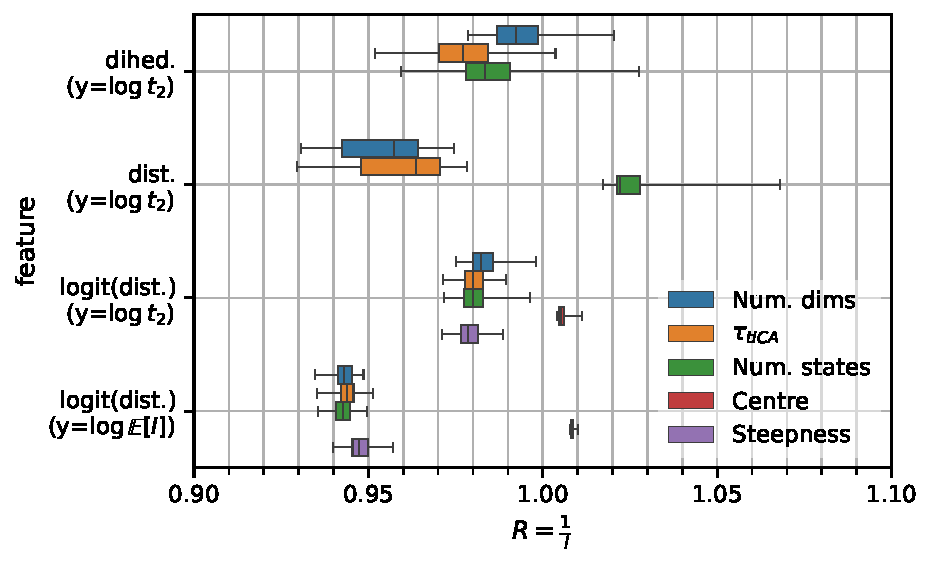
\includegraphics[width=0.8\textwidth]{figures/sensitivity.pdf}
% %     \caption{\textbf{Relevance of hyperparameters to the implied timescales and expected improvement.} The hyperparameter relevance ($R$) to the timescales ($y=\log{t_{2}}$) for the three different features,  and the expected improvement ($y=\log{\mathbb{E}[I]}$) for the logistic-distances feature. The larger the relevance, the more sensitive the outcome is to each hyperparameter.  The relevance is calculated from the learned kernel parameters of the relevant Gaussian process. Box plots show the distribution of values from \num{100} bootstrap samples. The relevance $R$ is the inverse of the characteristic length-scale of the exponential kernel in equation~\ref{eqn:kern_exp}. }
% %     \label{fig:sensitivity}
% % \end{figure}

% In order to understand the timescale distribution we estimate the sensitivity of the timescales to the hyperparameters. Previous work has shown that the type of feature used is important in determining the eigenvector accuracy. This is consistent with figure~\ref{fig:1fme_timescales}  where the majority of the best hyperparameters use the `logit(dist.)' feature.  However, figure~\ref{fig:ts_distribution} also shows that a) there is significant overlap of the timescale distributions for each feature, and b) the best performing feature also gives rise to the worst performing models. The type of feature is therefore a necessary but not sufficient hyperparameter to tune in order to maximize the timescales. It is important, therefore, to consider the remaining hyperparameters (e.g., the TICA lag time, TICA dimension etc.) and how they affect the timescales.  

% We estimate the sensitivity of the remaining hyperparameters for each feature by modelling $\log{t_{2}}$ as a Gaussian process as a function of the MSM hyperparameters. This model of the response of the $t_2$ to variation in the hyperparameters we call a \emph{response surface}. The covariance function that gave the best fitting model used the fully additive structure, equation~\ref{eqn:plus_kernel}, with an exponential kernel over each hyperparameters, equation~\ref{eqn:kern_exp}. 

% Figure~\ref{fig:sensitivity} plots the  the relevance of hyperparameters, $R$, in determining $t_{2}$. It shows that the hyperparameters vary in how important they are in determining $t_2$ for each different feature.  For the `dihed.' feature it shows that the TICA dimension, lag time and number of microstates are all equally relevant in determining $t_2$, however $t_2$ does not vary greatly with changes in any of these hyperparameters (as $R\simeq 1$). For the `dist.' feature the number of microstates is the most relevant in determining $t_2$. For the `logit(dist.)' feature the location of the centre of the logistic function (as this feature is a continuous approximation to a contact map, the `centre' corresponds  to the contact map cut-off) is the most important hyperparameter. The fitted Gaussian process regression models which give rise these values are shown in the supplementary material figures~\ref{fig:repsonse_diheds}, \ref{fig:repsonse_dist}, and \ref{fig:repsonse_logistic}. 

% Why is the hyperparameter sensitivity important? First, as has been  previously shown~\cite{bergstra_jamesbergstra_random_2012}, if all hyperparameters have a large relevance ($R \gg 1$), then to finding the maximum of the response surface (i.e., the hyperparameters which give rise to the maximum $t_2$) is hard. In this case, it is important to try all combinations of hyperparameters i.e., a  grid-search strategy, or to employ an active learning approach~\cite{snoekAbstractBayesianOptimization2013}.  However, if only a small proportion of the hyperparameters have a high relevance then randomly sampling hyperparameters is the more efficient strategy.  Second, the lack of pattern in the relevance of hyperparameters indicates that it is not possible to draw general conclusions about hyperparameters, indicating that default values of hyperparameters may not be useful and that each system must optimized individually. 




% \begin{figure}
%     \centering
%     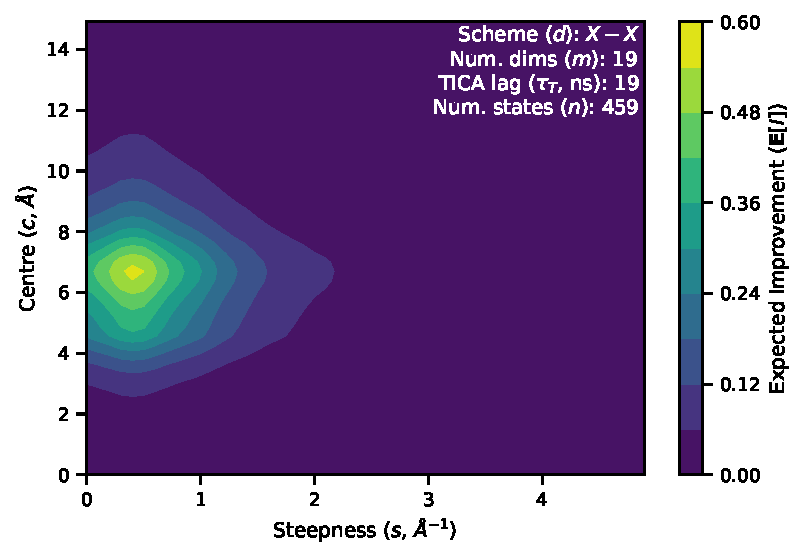
\includegraphics{figures/surface_distances_logistic_ei.pdf}
%     \caption{\textbf{Expected improvement as a function of the two most relevant hyperparameters - the logistic center ($c$) and steepness ($s$)}. The remaining hyperparameters take on the values shown in the annotation. These were chosen so as to maximize the expected improvement, i.e., the figure plots $y=f(s, c, d^{*}, m^{*}, \tau^{*}, n^{*})$ where $s^{*}, c^{*}, d^{*}, m^{*}, \tau^{*}, n^{*} = \argmax \left [f(s, c, d, m, \tau,n)\right]$. }
%     \label{fig:ei_surface}
% \end{figure}




% In order to check the convergence of the results shown in panel (a) of figure~\ref{fig:1fme_timescales} and to potentially improve the $t_2$ estimate,  we use a single round of Bayesian optimisation. To this end, we first calculate the expected improvement, $\mathbb{E}[I]$,  using the response surface calculated in the sensitivity analysis and  equation~\ref{eqn:ei_for_gp}. As the `logit(dist.)' feature has the best performing trials we optimise only this feature. 


% The expected improvement is shown in figure~\ref{fig:ei_surface} as a function of the `centre' and the `steepness' hyperparameters (the remaining hyperparameters are held at their values at the peak of expected improvement).  This shows that we expect any values of the `centre' and `steepness' hyperparameters to increase $t_2$ by at least \SI{2}{\micro\second} if the other hyperparameters take on their values in the annotation. However, with $c\simeq \SI{7}{\angstrom}$ and $s\simeq \SI{0.5}{\per\angstrom}$ we can expect an improvement in the timescales of almost $\SI{3}{\micro\second}$. 


% We then estimated MSMs using the five sets of hyperparameters with the largest expected improvement. The new optimized values of $t_2$ are shown in panel (b) of figure~\ref{fig:1fme_timescales}.  These clearly show that optimized models all have timescales slightly greater than the incumbent ($t_2 \simeq \SI{20}{\micro\second}$):  the optimized timescales range up to $t_2 \simeq \SI{24}{\micro\second}$, which are similar to the improvements predicted by the expected improvement function. The optimized hyperparameters differ slightly from the incumbent (except in the choice of distance scheme - all used the $\alpha$-carbon distances). We have, therefore, a set of six MSMs which differ slightly in the values of their hyperparameters, which all give similar implied timescales: we can be sure that our model is robust. 

% In order to check the validity of the optimized models, figure xx shows the metastable states of (a) the second ranked model from the unoptimized set (the second model in figure~\ref{fig:1fme_timescales}(a), $t_2 simeq \SI{9}{\micro\second}$), (b) the first ranked model from the unoptimized set (the first model in figure~\ref{fig:1fme_timescales}(a), $t_2 simeq \SI{20}{\micro\second}$) and (c) the optimized model (the first ranked model from the optimized set (the first model in figure~\ref{fig:1fme_timescales}(b), $t_2 simeq \SI{24}{\micro\second}$). 

% We can also ask ourselves whether we could improve our hyperparameters using Bayesian optimisation with less data. This is relevant if estimating the models is expensive. To answer this, we remove the incumbent in panel (b) from the hyperparameter trial data-set, re-estimated the response surface and expected improvement and sampled new hyperparameters. The new incumbent in this case was $t_2 = \simeq \SI{10}{\micro\second}$, shown in purple in panel (c) figure~\ref{fig:1fme_timescales}.  The new values of $t_2$,  are all improvements of up to \SI{10}{\micro\second}: the new timescales range up to $t_2 \simeq \SI{20}{\micro\second}$. It is therefore plausible that one may use Bayesian optimisation to optimize MSM hyperparameters, even when the timescale measurements are noisy and there are no strong dependence on any of hyperparameters.  



% \subsection{Sensitivity analysis}

% \textbf{Ryan}

% \begin{itemize}
%     \item Can you put the details about how exactly hyperparameter importance was measured.
%     \item should include calculation details and refer to the theory in previous section. 
%     \item I would do this first before the theory (so you don't include useless detail in the theory section). 
% \end{itemize}




 

% \subsubsection{Sensitivity Analysis}

% Sensitivity analysis is used to determine the dependency of model outputs on their inputs [uncertainty book]. This is a large research area and we refer the reader to [uncertainty book] and the references within for a full account.  In this work, we conduct a \emph{global sensitivity analysis} which looks at model outputs as a function of the whole input space. This is in contrast to a \emph{local sensitivity analysis} which look at  how small perturbations around a give set of inputs affect the outcomes.  Our simplified sensitivity analysis uses analysis of variance in conjunction with random forests to assess, as developed by Hutter et. al. \cite{hutter_efcient_nodate}.  


% \textbf{Ryan}:
% \begin{itemize}
%     \item Summarise the theory and method for assessing hyperparameter importance in Optunal. 
%     \item reference is: https://proceedings.mlr.press/v32/hutter14.html
%     \item Should be relatively brief (a few paragraphs) 
% \end{itemize}

